\documentclass{article}
\usepackage{graphicx}
\usepackage[utf8]{inputenc}
\usepackage{latexsym,amsfonts,amssymb,amsthm,amsmath}
\usepackage[a4paper,margin=1in]{geometry} % Adjust margins as needed
\usepackage{float}
\usepackage{hyperref}
\usepackage{caption}
\usepackage{subcaption} % For subfigures (modern alternative to subfigure)


\setlength{\parindent}{0in}
\setlength{\oddsidemargin}{0in}
\setlength{\textwidth}{6.5in}
\setlength{\textheight}{8.8in}
\setlength{\topmargin}{0in}
\setlength{\headheight}{18pt}




\begin{document}

	\begin{titlepage}
    	\vspace*{\fill} % Add space before the title block
    	\begin{center}
        	{\huge \textbf{CMU Fall24 16820 Homework 5} \par}
       		\vspace{0.5cm}
        		{\large Patrick Chen \par}
        		\vspace{0.5cm}
		%{\large Collaborators: NA \par}
		%\vspace{0.5cm}
        		{\large November 10, 2024 \par}
    	\end{center}
    	\vspace*{\fill} % Add space after the title block to center everything
	\end{titlepage}
	
	\newpage
	\subsection*{Q1-a at page 3}
	Ans:\\
	\hangindent=1.5em \hspace{1.5em}According to Lambertian's cosine law, the intensity of light observed from a Lambertian surface is propational to the cosine of the angle $\theta$ between the surface normal, $\vec{n}$, and the direction of the incoming light, $\vec{l}$.
	\begin{align}
		\mathbf{\overrightarrow{n}} \cdot \mathbf{\overrightarrow{l}} = |\mathbf{\overrightarrow{n}}| |\mathbf{\overrightarrow{l}}| \cos(\theta) 
	\end{align}
	Typically in the context of n-dot-l lighting, both $\vec{n}$ and $\vec{l}$ are unit vectors, so we have:
	\begin{align}
	\mathbf{\overrightarrow{n}} \cdot \mathbf{\overrightarrow{l}} = \cos(\theta) 
	\end{align}
	As shown in Fig. 2a as below, the $\theta$ is the dot product between $\vec{n}$ and $\vec{l}$. The dot product, $\theta$, quantifies the amount of incident light that is effectively contributing to the brightness of the surface. As the angle increases, less light is effectively reaching the surface, as the angle decrease, more light hits the surface, reaching maximum incoming light when $\theta$ is 0, identical to the case that $\vec{l}$ is aligned with $\vec{n}$.
	
	\begin{minipage}{0.48\linewidth}
	\centering
	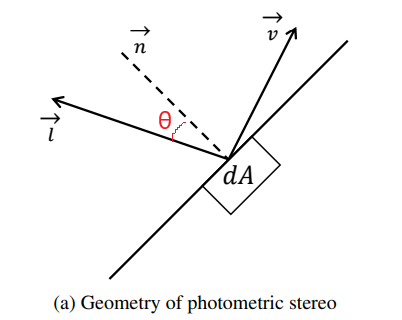
\includegraphics[width=\linewidth]{./Q1_a.png}
	\refstepcounter{figure}  % Increment the figure counter
	\textbf{Fig. 2a} % Manually add a caption/title
	\label{fig:Q1_a}         % Label for referencing	
	\end{minipage}
	\hfill
	\begin{minipage}{0.48\linewidth}
	\centering
	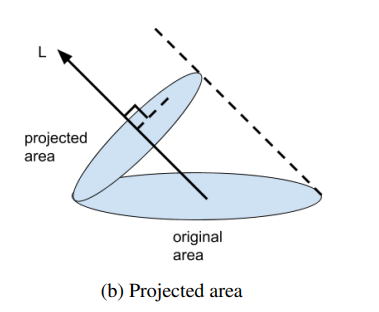
\includegraphics[width=\linewidth]{./Q1_b.png}
	\refstepcounter{figure}  % Increment the figure counter
	\textbf{Fig. 2b} % Manually add a caption/title
	\label{fig:Q1_b}         % Label for referencing
	\end{minipage}	
	\newline
	
	\hangindent=1.5em \hspace{1.5em}The projected area, $\mathbf{dA_{projected}}$, in Fig. 2b is the original area, $\mathbf{dA}$, times $\cos(\theta)$:
	\begin{align}
		\mathbf{dA_{projected}} &= \mathbf{dA} \cdot \cos(\theta) \\
								&= \mathbf{dA} \cdot \mathbf{\overrightarrow{n}} \cdot \mathbf{\overrightarrow{l}} \\
		\frac{\mathbf{dA_{projected}}}{\mathbf{dA}} &= \cos(\theta) \\
													&= \mathbf{\overrightarrow{n}} \cdot \mathbf{\overrightarrow{l}}
	\end{align}
	As $\theta$ becomes larger, the effective area that light directly expose to becomes smaller, and on the opposite, as $\theta$ becomes smaller, the effective area becomes larger, reaching maximum $\mathbf{dA}$ as $\theta$ = 0. Hence, the projected area comes into the equation as part of the Lambertian reflectance model through the $\cos(\theta)$ factor.
	\newline
	
	\hangindent=1.5em \hspace{1.5em}The reason that the viewing direction does not matter is that we assume the surface is Lambertial surface, which reflects light equally in all directions, $\vec{v}$. Specifically, the light reflected from each point on the surface has the same intensity value no matter where the observer is located. It also means that the intensity of light that the observer can observe is based solely on the $\vec{n} \cdot \vec{l} = \cos(\theta)$ term.

	\newpage
	
	\newpage
	\subsection*{Q1-b at page 4}
	Ans:\\
	\hangindent=1.5em \hspace{1.5em}Following \autoref{fig:Q1_b_a} - \autoref{fig:Q1_b_c} shows the rendered result, and the \autoref{fig:Q1_b_cns} shows the code snippet in q1.py.
	\newline
	
	\begin{minipage}{0.31\linewidth}
	\centering
	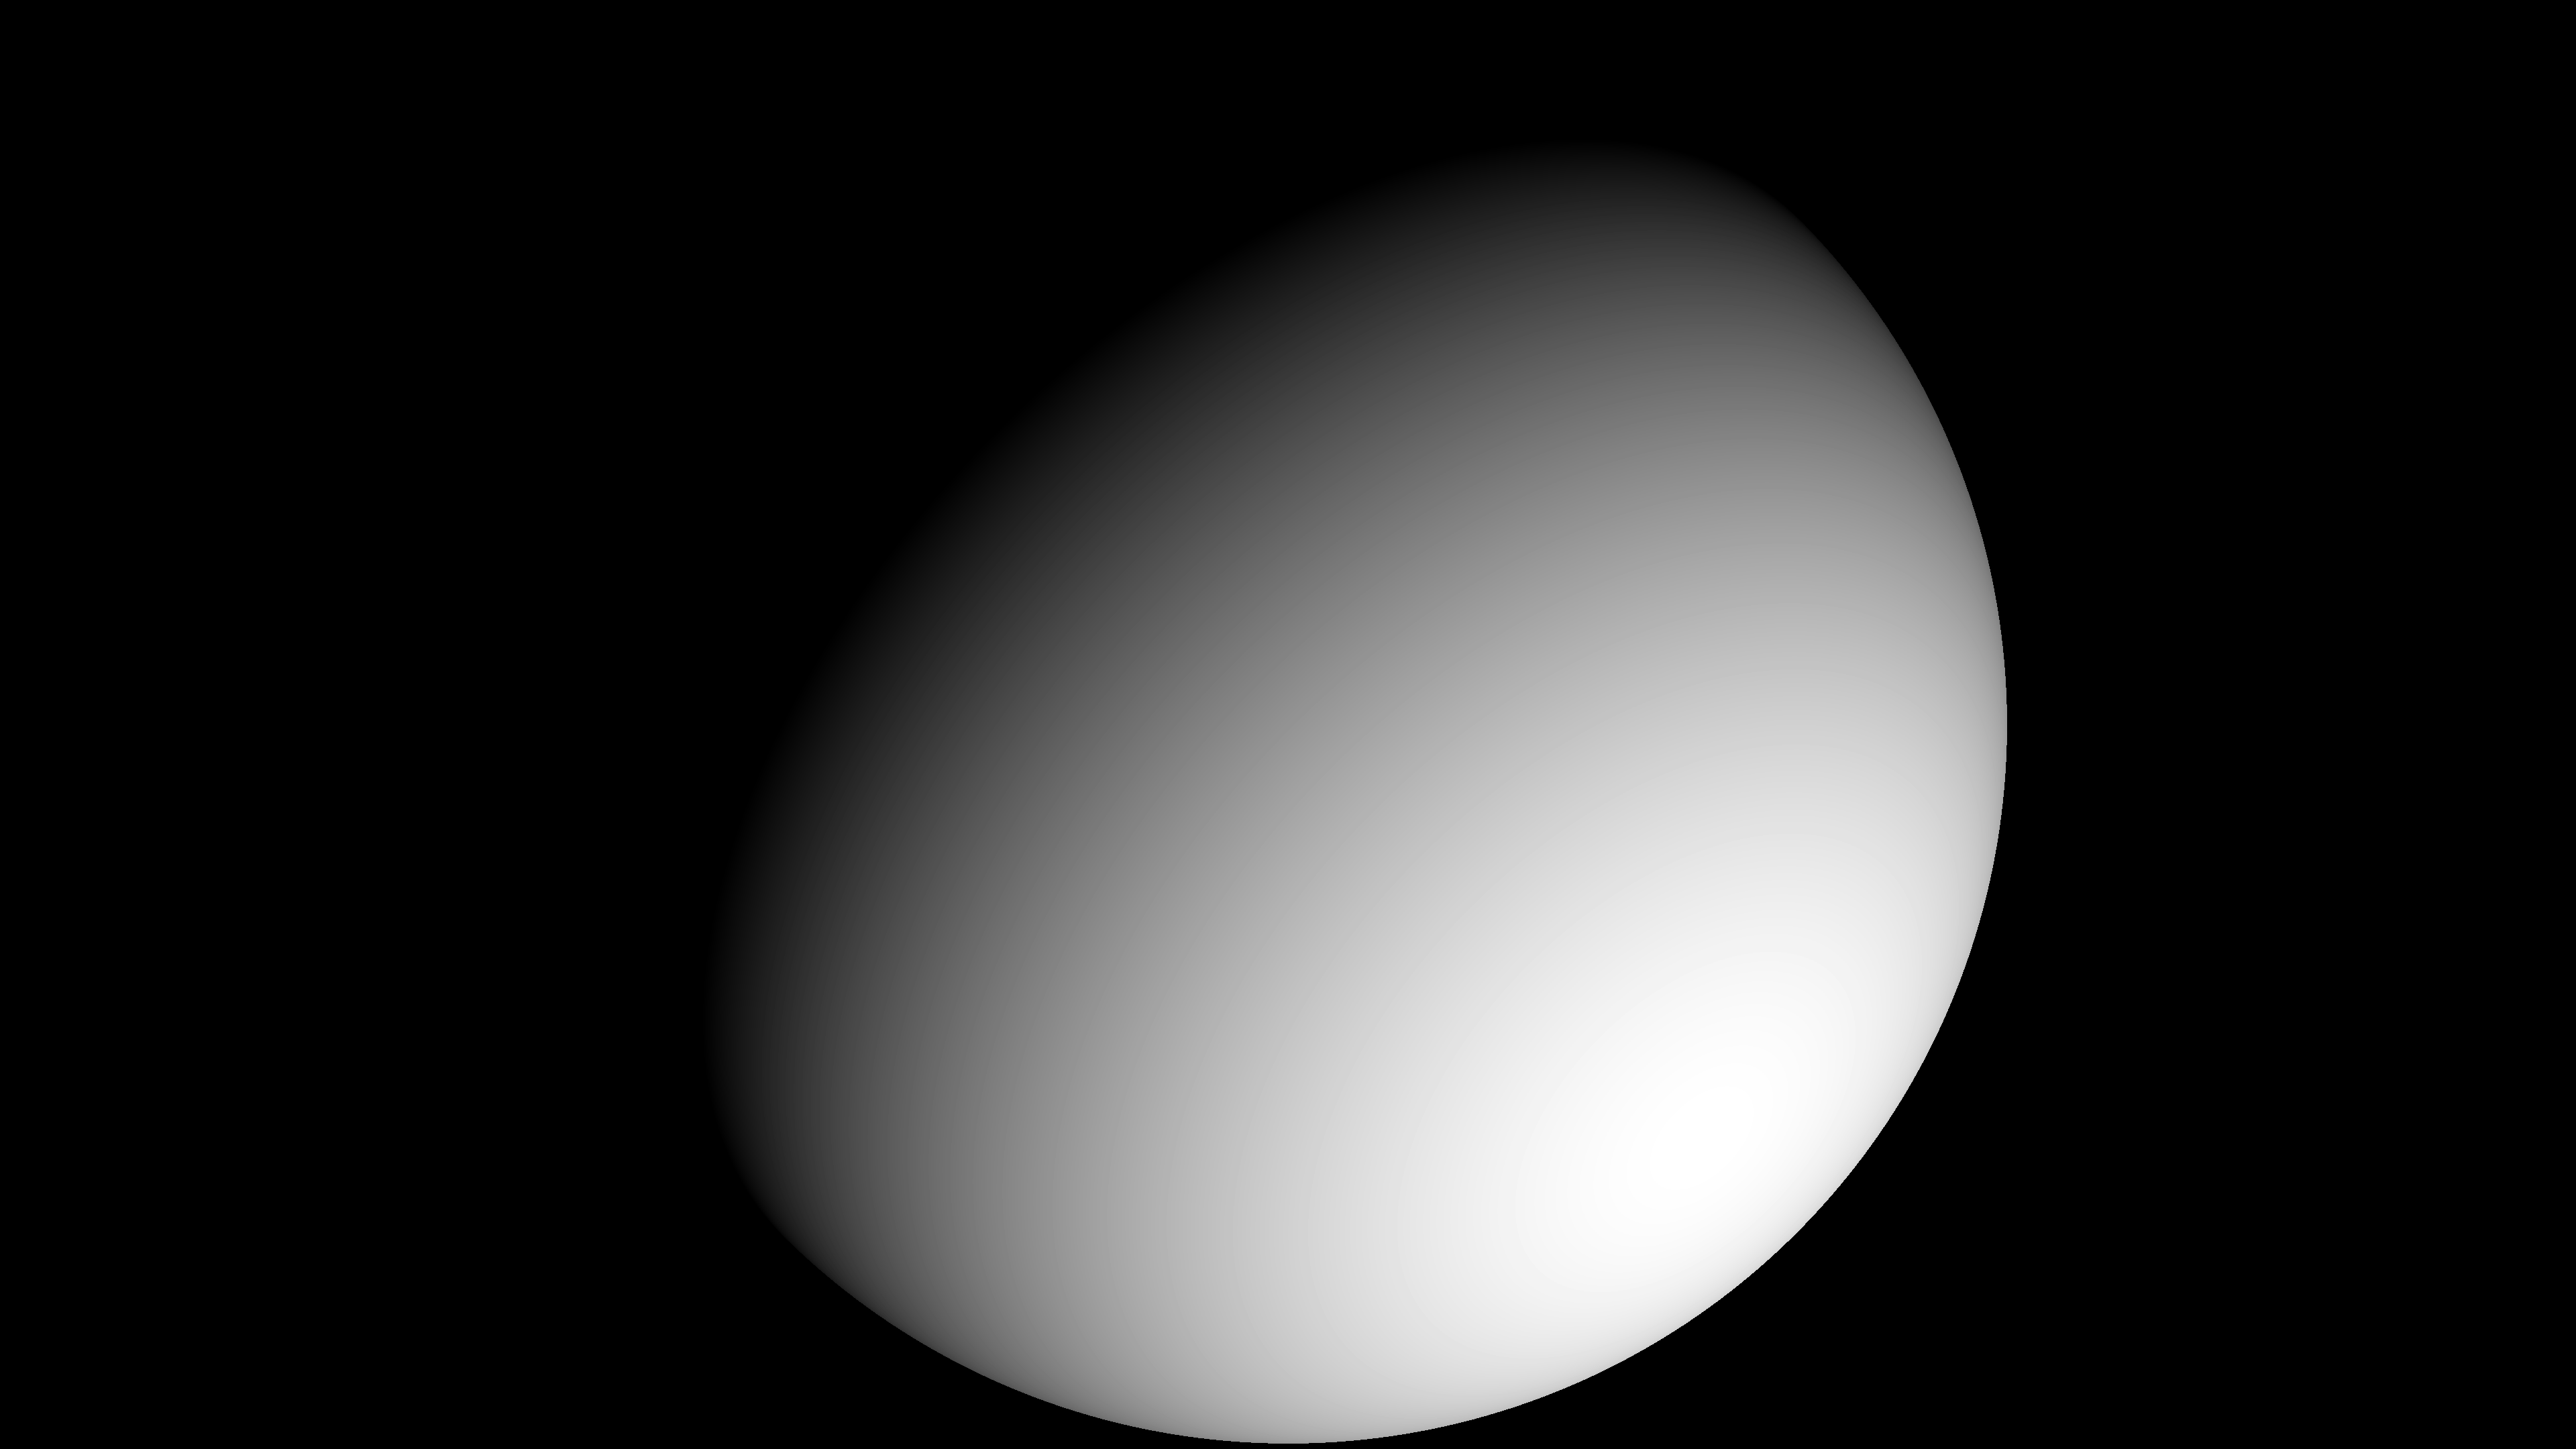
\includegraphics[width=\linewidth]{./src/1b-a.png}
	\refstepcounter{figure}  % Increment the figure counter
	\textbf{Figure \thefigure:} Rendered Result with (1, 1, 1)/$\sqrt{3}$ Light Vector  % Manually add a caption/title
	\label{fig:Q1_b_a}         % Label for referencing	
	\end{minipage}
\hfill
	\begin{minipage}{0.31\linewidth}
	\centering
	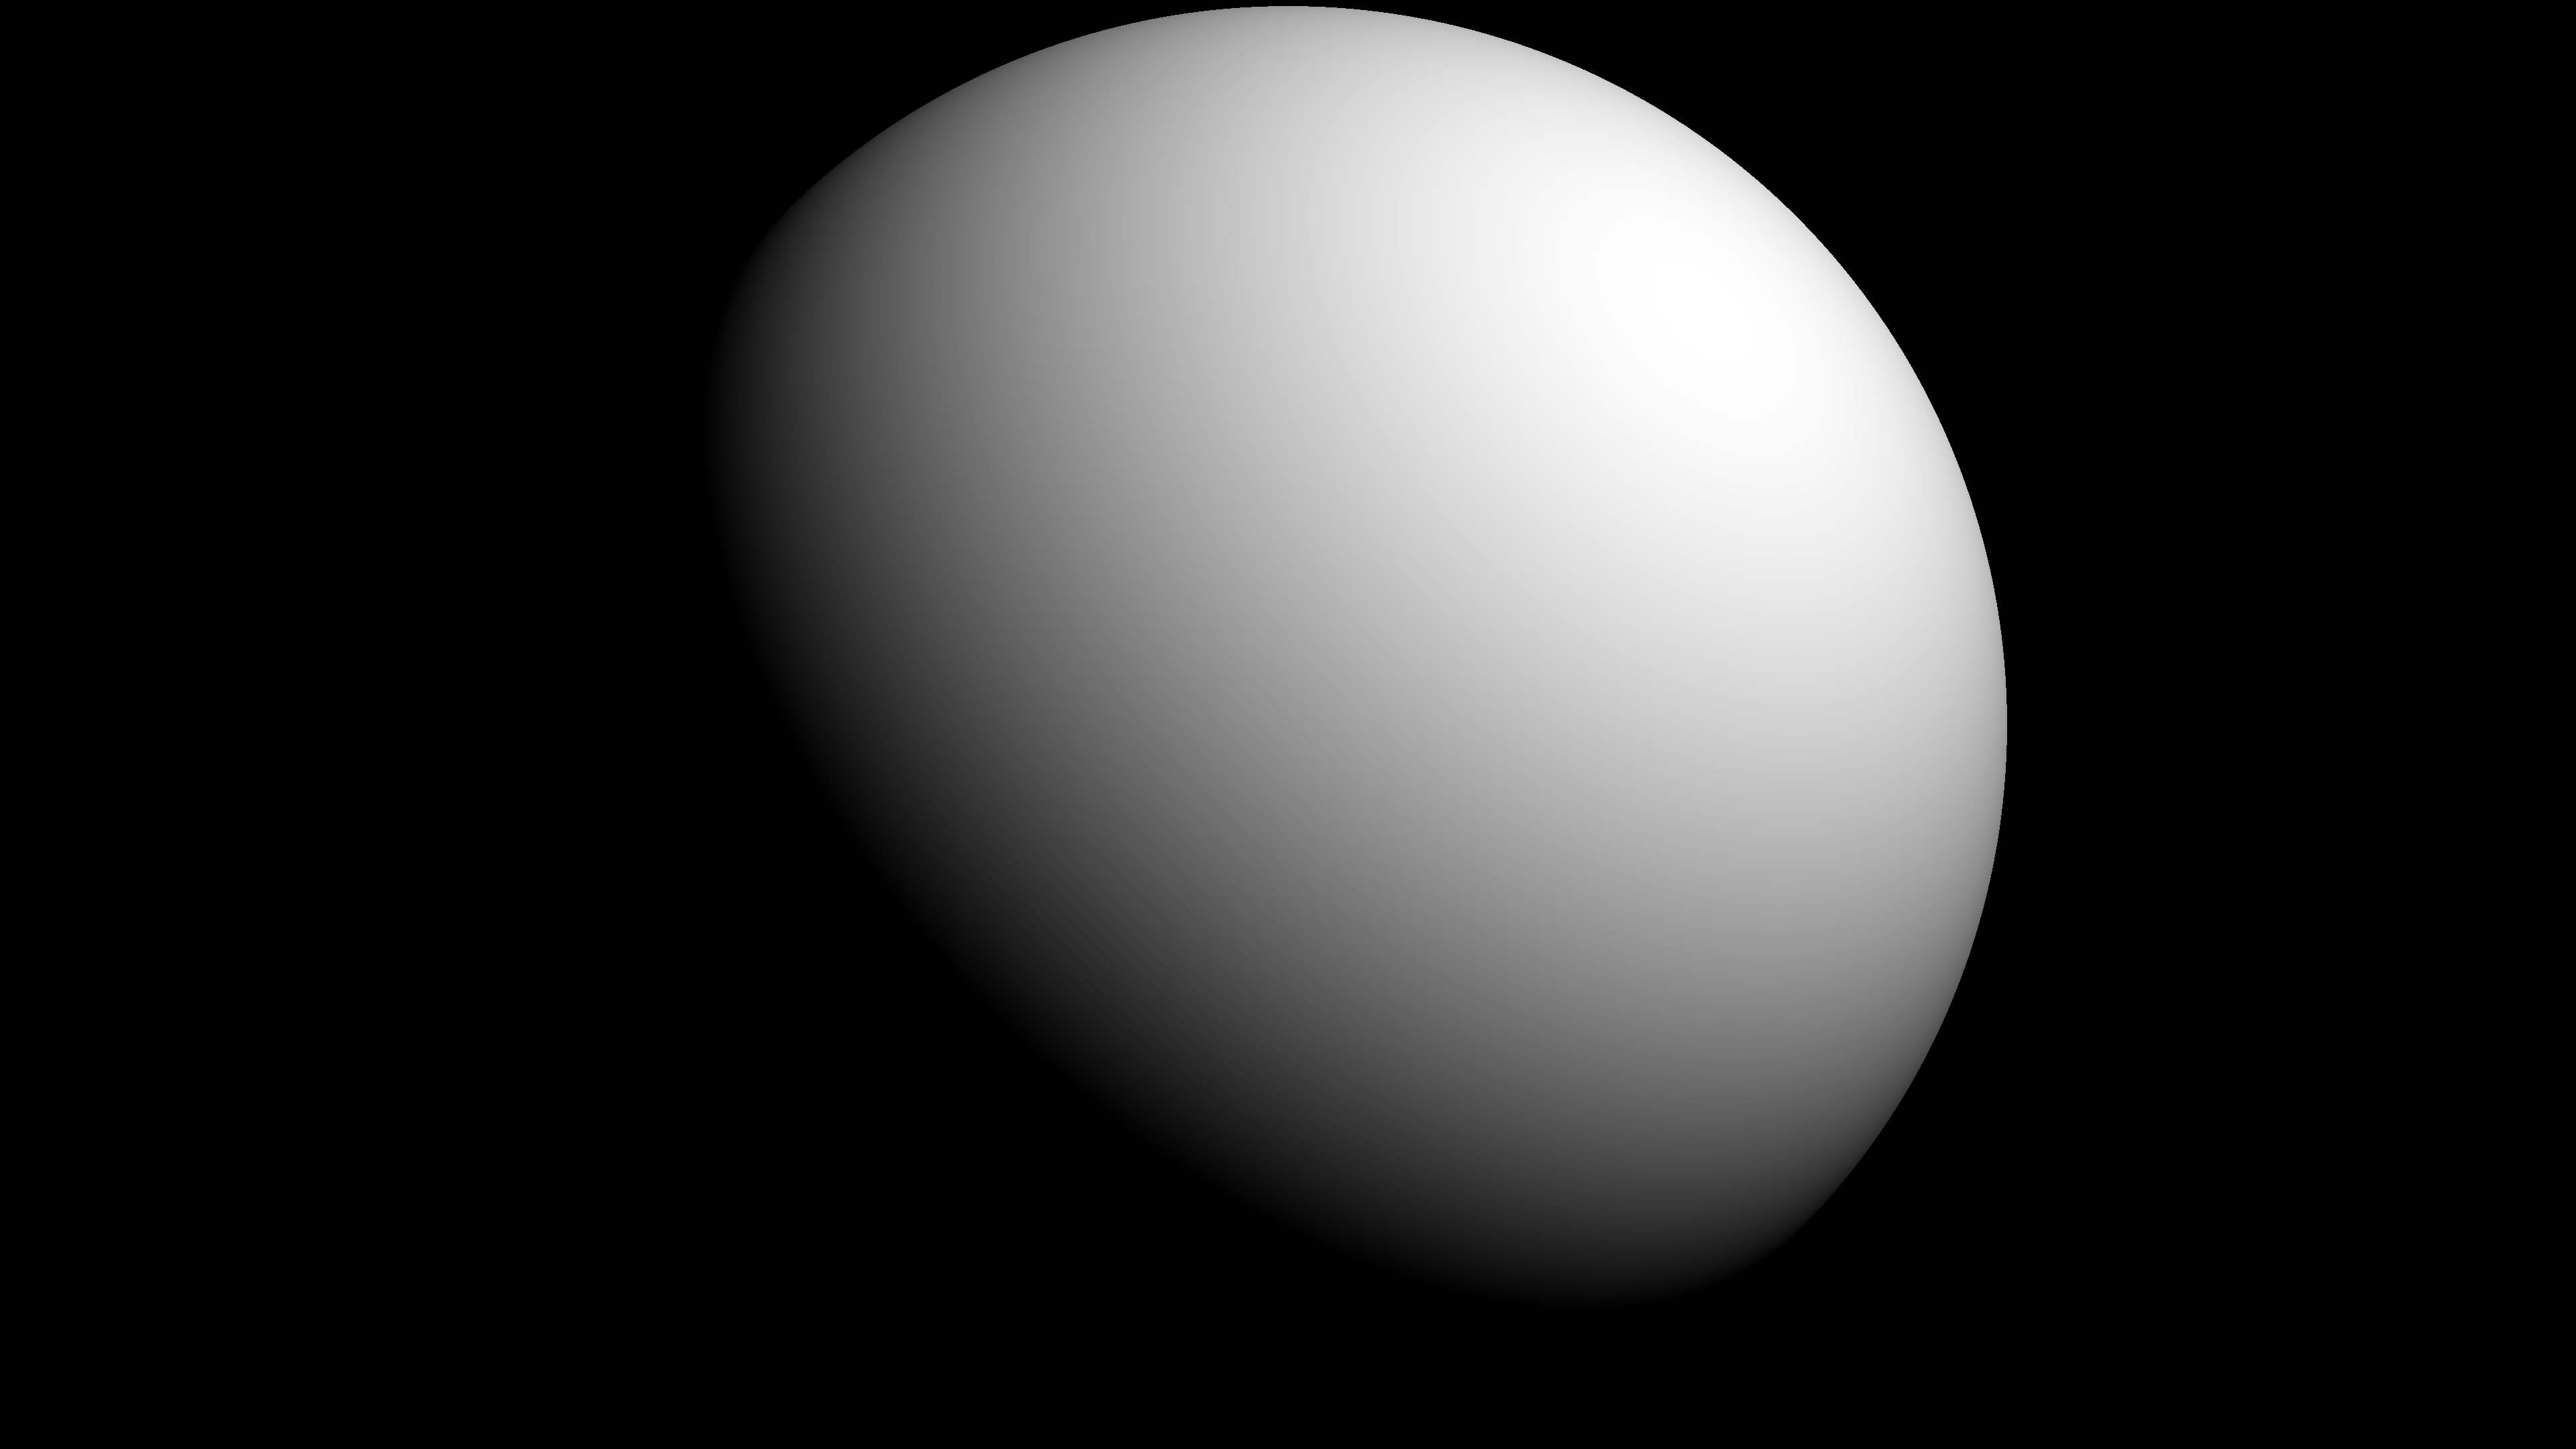
\includegraphics[width=\linewidth]{./src/1b-b.png}
	\refstepcounter{figure}  % Increment the figure counter
	\textbf{Figure \thefigure:} Rendered Result with (1, -1, 1)/$\sqrt{3}$ Light Vector  % Manually add a caption/title
	\label{fig:Q1_b_b}         % Label for referencing
	\end{minipage}	
\hfill
	\begin{minipage}{0.31\linewidth}
	\centering
	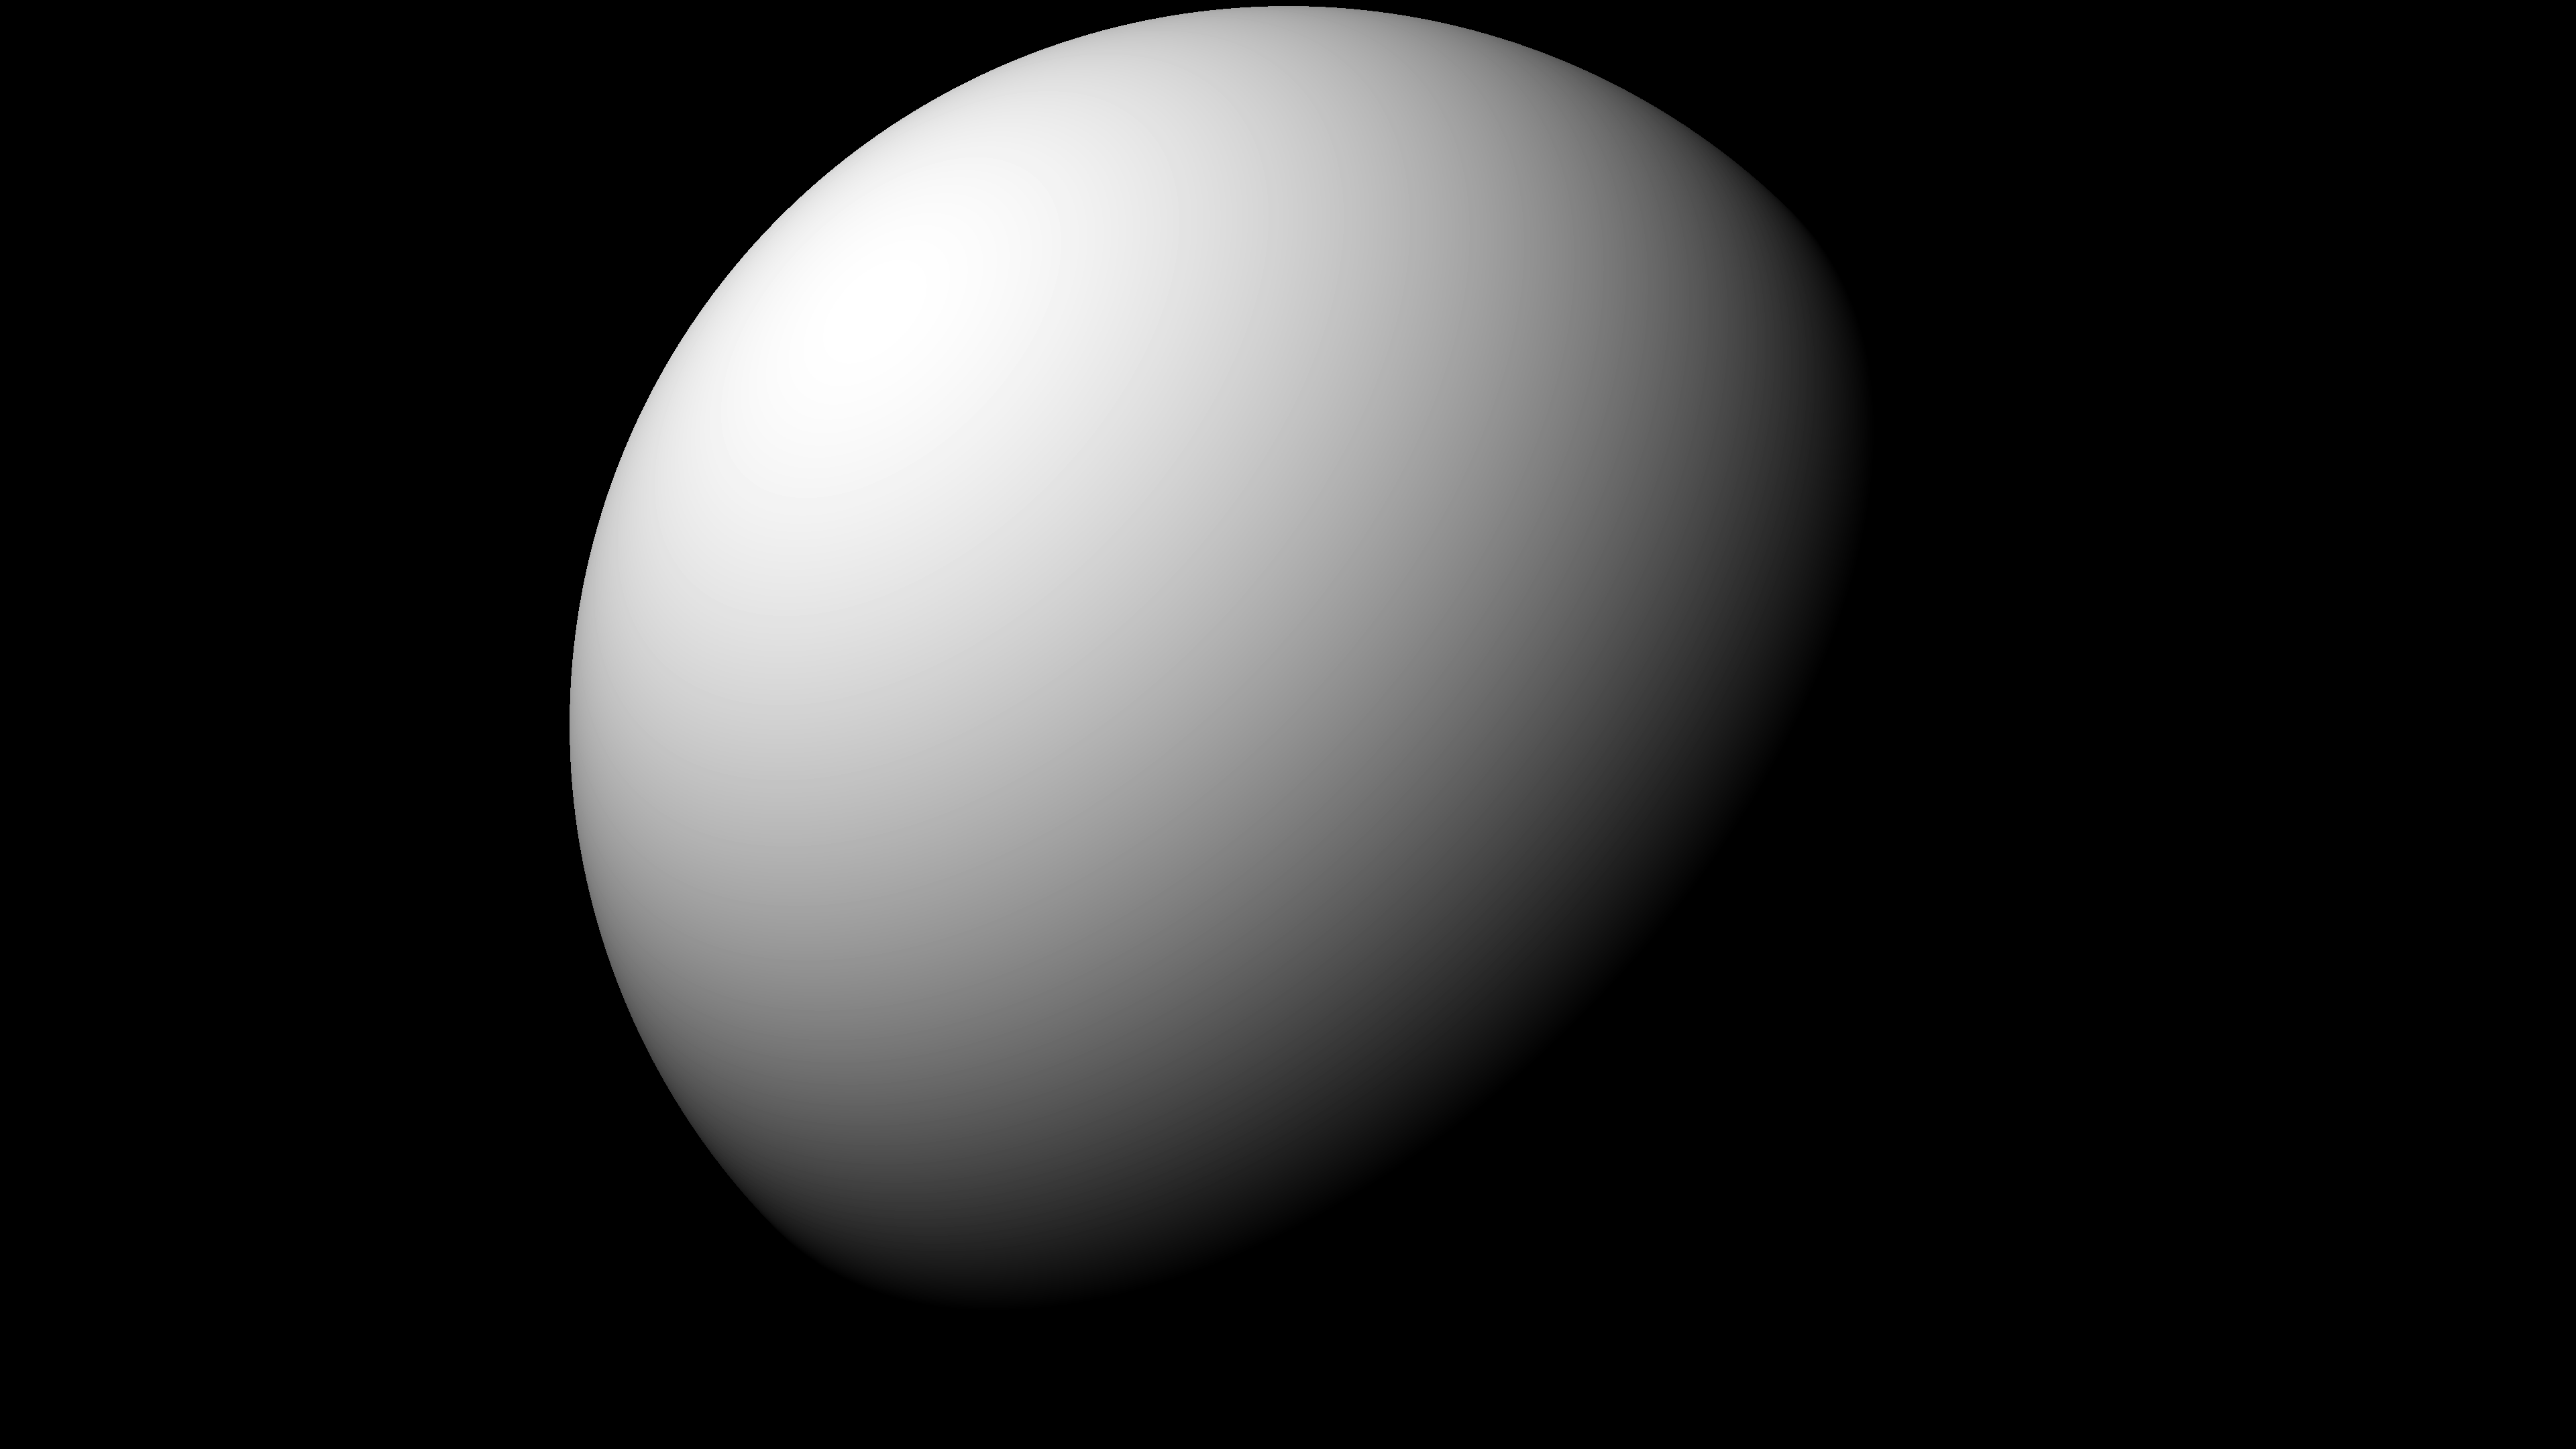
\includegraphics[width=\linewidth]{./src/1b-c.png}
	\refstepcounter{figure}  % Increment the figure counter
	\textbf{Figure \thefigure:} Rendered Result with (-1, -1, 1)/$\sqrt{3}$ Light Vector  % Manually add a caption/title
	\label{fig:Q1_b_c}         % Label for referencing
	\end{minipage}	
	\newline
	\newline

	\begin{minipage}{1\linewidth}
	\centering
	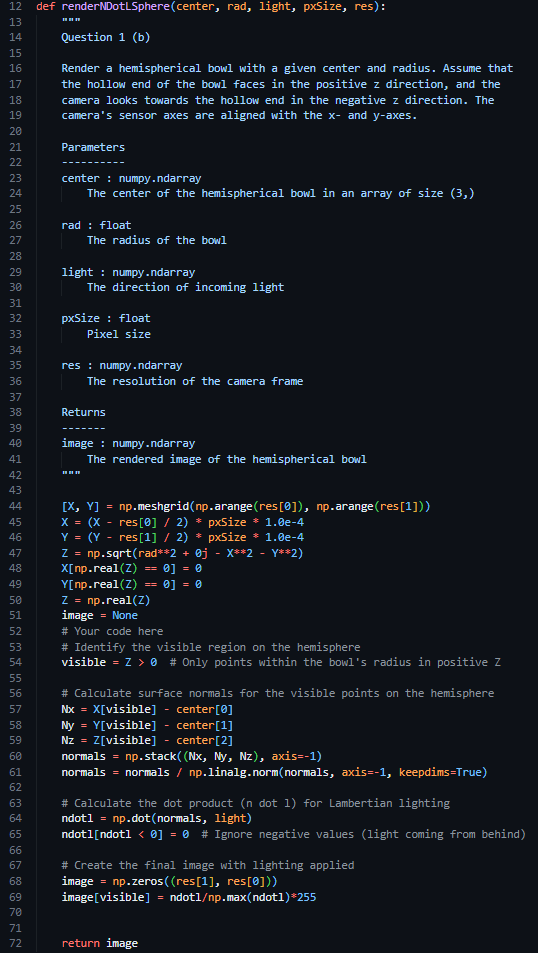
\includegraphics[width=0.7\linewidth, height=0.95\columnwidth]{./Q1_b_cns.png}
	\refstepcounter{figure}  \\% Increment the figure counter
	\textbf{Figure \thefigure:} Code Snippet  % Manually add a caption/title
	\label{fig:Q1_b_cns}         % Label for referencing
	\end{minipage}	
	
	\newpage
	\subsection*{Q1-c at page 4}
	Ans:\\
	\hangindent=1.5em \hspace{1.5em}Following \autoref{fig:Q1_c_cns} shows the conde snippet of loadData() in q1.py.
	\newline
	
	\begin{minipage}{1\linewidth}
	\centering
	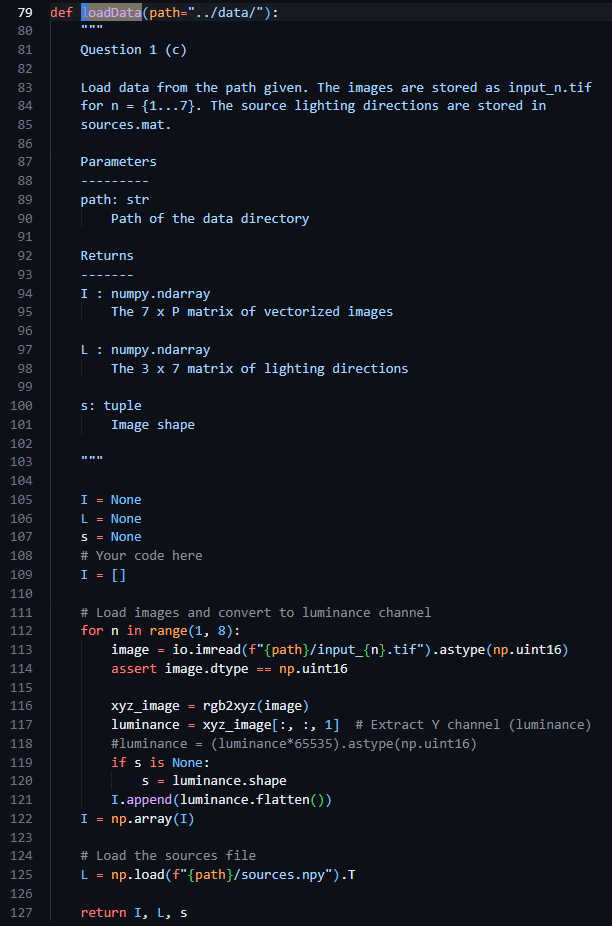
\includegraphics[width=0.7\linewidth, height=0.95\columnwidth]{./Q1_c_cns.png}
	\refstepcounter{figure}  \\% Increment the figure counter
	\textbf{Figure \thefigure:} Code Snippet  % Manually add a caption/title
	\label{fig:Q1_c_cns}         % Label for referencing
	\end{minipage}
	
	\newpage
	\subsection*{Q1-d at page 4}
	Ans:\\
	\hangindent=1.5em \hspace{1.5em} $L^{T}$ has the shape (7, 3), representing the transposed light directions. If L has rank of 3, it means 3 of the light directions in L can span the whole 3-dimensional space. Also, $B$ has the shape of (3, P), representing the set of pseudonormals in the images. If B has rank 3, it means 3 of the pseudonormals in B could span the whole 3-dimensional space. If both L and B have rank of 3, then $I = L^TB$ would also have rank 3, meaning that the singular value of I should agree with rank 3.\newline
	However, we can see from below \autoref{fig:Q1_d_res}, the singular value shows that I has rank of 7, not agreeing with rank-3 requirement. It is because that if the light directions in L or the pseudonormals in B are not linearly independent, due to the noise or measurement imprecision of light on camera intensity, then the rank of L and B might not be exactly 3, resulting in the disagreement here. The \autoref{fig:Q1_d_cns} shows the conde snippet in q1.py.
	\newline
	
	\begin{minipage}{1\linewidth}
	\centering
	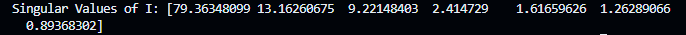
\includegraphics{./Q1_d_res.png}
	\refstepcounter{figure}  \\% Increment the figure counter
	\textbf{Figure \thefigure:} Singular Values of I  % Manually add a caption/title
	\label{fig:Q1_d_res}         % Label for referencing
	\end{minipage}
	\newline
	\newline
	
	\begin{minipage}{1\linewidth}
	\centering
	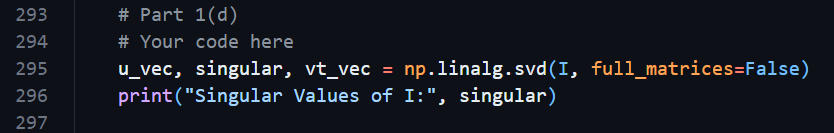
\includegraphics[width=0.8\columnwidth]{./Q1_d_cns.png}
	\refstepcounter{figure}  \\% Increment the figure counter
	\textbf{Figure \thefigure:} Code Snippet of (d)  % Manually add a caption/title
	\label{fig:Q1_d_cns}         % Label for referencing
	\end{minipage}	
	
	\newpage
	\subsection*{Q1-e at page 4}
	Ans:\\
	\hangindent=1.5em \hspace{1.5em} The way I construct A and B is shown in the following derivation of estimated B:
	\begin{align}
		\mathbf{I} &= \mathbf{L^{T}}\mathbf{B} \\
		Set \hspace{1mm} \mathbf{A} &= L^{T}, \mathbf{x} = \mathbf{B}, \mathbf{y} = \mathbf{I} \\
		\rightarrow \mathbf{A}\mathbf{x} &= \mathbf{y} \\
		\rightarrow \mathbf{x} &= (\mathbf{A^T}\mathbf{A})^{-1}\mathbf{A^T}\mathbf{y} \\
		\rightarrow \mathbf{B} &= (\mathbf{L}\mathbf{L^T})^{-1}\mathbf{L}\mathbf{I} 
	\end{align}
	Following \autoref{fig:Q1_e_cns} shows the code snippet of (e) in q1.py.
	\newline
	
	\begin{minipage}{1\linewidth}
	\centering
	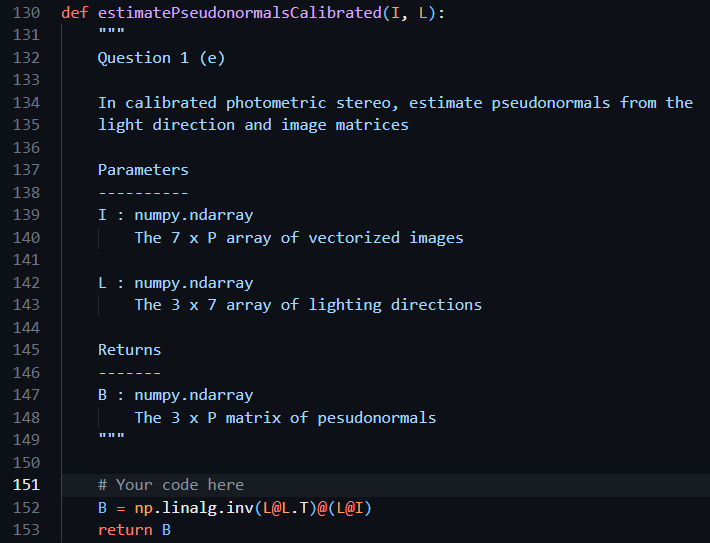
\includegraphics[width=0.5\columnwidth, height=0.4\linewidth]{./Q1_e_cns.png}
	\refstepcounter{figure}  \\% Increment the figure counter
	\textbf{Figure \thefigure:} Code Snippet of (e)  % Manually add a caption/title
	\label{fig:Q1_e_cns}         % Label for referencing
	\end{minipage}	
	
	\newpage
	\subsection*{Q1-f at page 5}
	Ans:\\
	\hangindent=1.5em \hspace{1.5em} The \autoref{fig:Q1_fa} and \autoref{fig:Q1_fb} show the result of estimated albedo and normals image respectively. The albedo image shows the reflectance of the face, and normal image shows the normal directions of the face. The forehead and cheek has smooth color changing, meaning there exist smooth change of normal direction among these areas, while the area like nose and lips show sharp change of color like boundaries, indicating the normal has sharp change among these areas. As of the albedo image, the forehead, cheek, nose, and ears show high intensity, indicating these areas have high reflectance property, aligning with my expectation because the skin of these area are usually shiny and oily. The \autoref{fig:Q1_f_cns1} and \autoref{fig:Q1_f_cns2} show the code snippets in q1.py.
	\newline
	
	\begin{minipage}{0.48\linewidth}
	\centering
	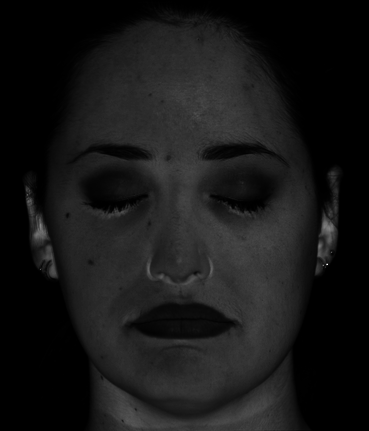
\includegraphics[width=\linewidth]{./src/1f-a.png}
	\refstepcounter{figure} \\ % Increment the figure counter
	\textbf{Figure \thefigure:} Estimated albedo  % Manually add a caption/title
	\label{fig:Q1_fa}         % Label for referencing	
	\end{minipage}
\hfill
	\begin{minipage}{0.48\linewidth}
	\centering
	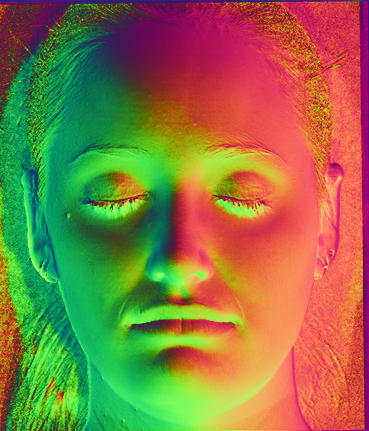
\includegraphics[width=\linewidth]{./src/1f-b.png}
	\refstepcounter{figure} \\ % Increment the figure counter
	\textbf{Figure \thefigure:} Estimated normals  % Manually add a caption/title
	\label{fig:Q1_fb}         % Label for referencing
	\end{minipage}	
\newline	
\newline

	\begin{minipage}{0.48\linewidth}
	\centering
	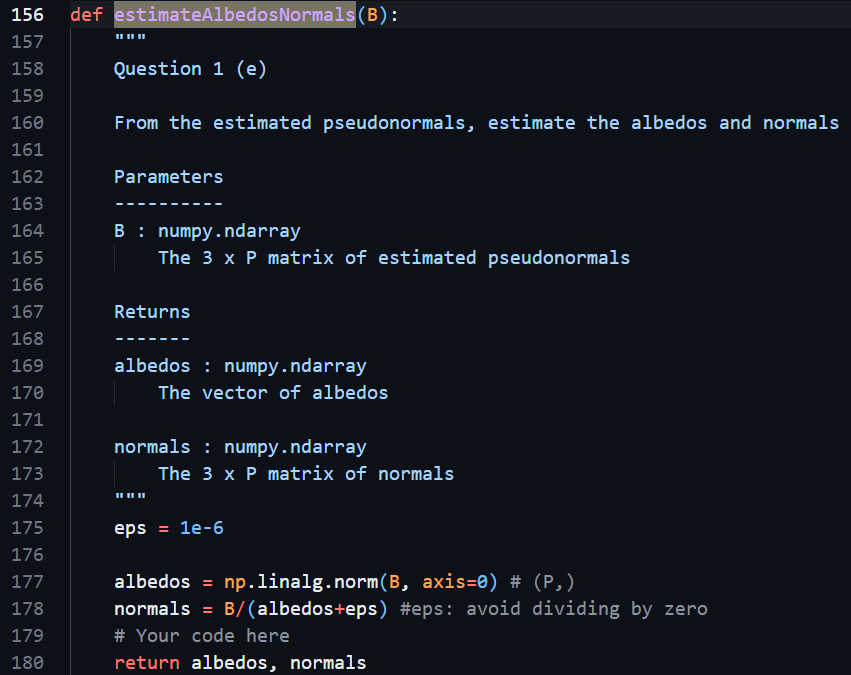
\includegraphics[width=\linewidth]{./Q1_f_cns1.png}
	\refstepcounter{figure} \\ % Increment the figure counter
	\textbf{Figure \thefigure:} Code Snippet of estimateAlbedosNormals()  % Manually add a caption/title
	\label{fig:Q1_f_cns1}         % Label for referencing	
	\end{minipage}
\hfill
	\begin{minipage}{0.48\linewidth}
	\centering
	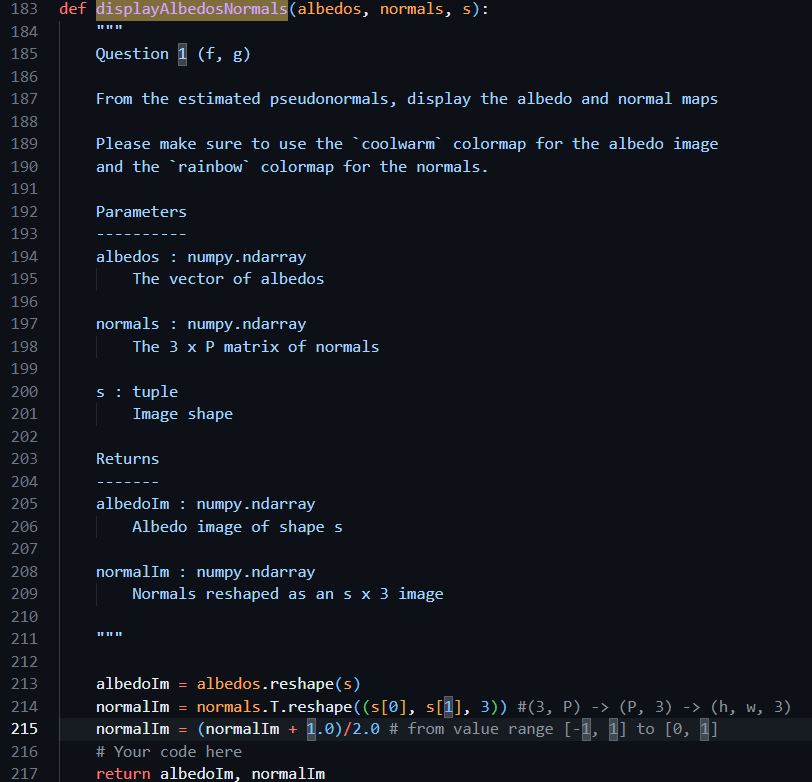
\includegraphics[width=\linewidth]{./Q1_f_cns2.png}
	\refstepcounter{figure} \\ % Increment the figure counter
	\textbf{Figure \thefigure:} Code Snippet of displayAlbedosNormals()  % Manually add a caption/title
	\label{fig:Q1_f_cns2}         % Label for referencing
	\end{minipage}	
\newline	

	\newpage
	\subsection*{Q1-g at page 5}
	Ans:\\
	\hangindent=1.5em \hspace{1.5em} The surface normal at point(x, y) is n = ($n_1, n_2, n_3$), and 3D depth map function at this point is z = f(x, y). We can have the tangent along x direction as: (1, 0, $\frac{\partial f(x, y)}{\partial x}$), and tangent along y direction as (0, 1, $\frac{\partial f(x, y)}{\partial y}$). Then the tangent x has the following relationship with normal n vector: \\
	\begin{align}
	&\mathbf{tangent}_x \cdot \mathbf{n} = (1, 0, \frac{\partial f(x, y)}{\partial x}) \cdot (n_1, n_2, n_3) = 0 \\
	&\rightarrow n_1 + n_3 \frac{\partial f(x, y)}{\partial x} = 0 \\
	&\rightarrow -\frac{n_1}{n_3} = \frac{\partial f(x, y)}{\partial x} = f_x
	\end{align}
	\vspace{1em}
	We can do the similar thing on the tangent y vector with normal n vector: \\
	\begin{align}
	&\mathbf{tangent}_y \cdot \mathbf{n} = (0, 1, \frac{\partial f(x, y)}{\partial y}) \cdot (n_1, n_2, n_3) = 0 \\
	&\rightarrow n_2 + n_3 \frac{\partial f(x, y)}{\partial y} = 0 \\
	&\rightarrow -\frac{n_2}{n_3} = \frac{\partial f(x, y)}{\partial y} = f_y
	\end{align}
	As one can see, the equation holds as the statement in Q1-g in hw5.pdf.
	
	\newpage
	\subsection*{Q1-h at page 6}
	Ans:\\
	\hangindent=1.5em \hspace{1.5em} We have the following two gradient calculations:
	\begin{align}
		g_x(x_i, y_j) &= g(x_{i+1}, y_j) - g(x_i, y_j) \\
		g_y(x_i, y_j) &= g(x_i, y_{j+1}) - g(x_i, y_j)
	\end{align}
	When using equation (18), the gradient of x, $g_x$, is:
	\[
	g_x =
	\begin{bmatrix}
		1 & 1 & 1 \\
		1 & 1 & 1 \\
		1 & 1 & 1 \\
		1 & 1 & 1
	\end{bmatrix}
	\]	
	When using equation (19), the gradient of y, $g_y$, is:
	\[
	g_y =
	\begin{bmatrix}
		4 & 4 & 4 & 4\\
		4 & 4 & 4 & 4 \\
		4 & 4 & 4 & 4 
	\end{bmatrix}
	\]	
	Method 1. Given g(0, 0) = 1, use $g_x$ to construct the first row of g, then use $g_y$ to construct the rest of g: \\
	Step1. Use $g_x$ to construct the first row: g(0, j) = g(0, j-1) + $g_x$(0, j-1), $1\leq j \leq 3$, the order is from left to right.
	\[
	g =
	\begin{bmatrix}
		1 & 2 & 3 & 4 \\
		0 & 0 & 0 & 0 \\
		0 & 0 & 0 & 0 \\
		0 & 0 & 0 & 0
	\end{bmatrix}
	\]
	Step2. Use $g_y$ for the rest: g(i, j) = g(i-1, j) + $g_y$(i-1, j), $1\leq i \leq 3$, $0\leq j \leq 3$, the order is from top to down. The reconstructed g is:
	\[
	g =
	\begin{bmatrix}
		1 & 2 & 3 & 4 \\
		5 & 6 & 7 & 8 \\
		9 & 10 & 11 & 12 \\
		13 & 14 & 15 & 16
	\end{bmatrix}
	\]	
	Method 2. Given g(0, 0) = 1, use $g_y$ to construct the first column of g, then use $g_x$ to construct the rest of g: \\
	Step1. Use $g_y$ to construct the first column: g(i, 0) = g(i-1, 0) + $g_y$(i-1, 0), $1\leq i \leq 3$, the order is from top to down.
	\[
	g =	
	\begin{bmatrix}
		1 & 0 & 0 & 0 \\
		5 & 0 & 0 & 0 \\
		9 & 0 & 0 & 0 \\
		13 & 0 & 0 & 0
	\end{bmatrix}
	\]
	Step2. Use $g_x$ for the rest: g(i, j) = g(i, j-1) + $g_x$(i, j-1), $0\leq i \leq 3$, $1\leq j \leq 3$, the order is from left to right. The reconstructed g is:
	\[
	g =
	\begin{bmatrix}
		1 & 2 & 3 & 4 \\
		5 & 6 & 7 & 8 \\
		9 & 10 & 11 & 12 \\
		13 & 14 & 15 & 16
	\end{bmatrix}
	\]	
	As we can see above, both procedures produce the same reconstruction of g.\\
	The integrability implies that:
	\begin{align}
	\frac{\partial g_x}{\partial y} = \frac{\partial g_y}{\partial x}
	\end{align}	
	So, we can modify the $g_x$ and $g_y$ as below to make them non-integrable:
	\[
	g_x =
	\begin{bmatrix}
		1 & 1 & 1 \\
		1 & 1 & 1 \\
		1 & 30 & 1 \\
		1 & 1 & 1
	\end{bmatrix}
	\]
	\[
	g_y =
	\begin{bmatrix}
		4 & 4 & 7 & 4\\
		4 & 4 & 4 & 4 \\
		4 & 4 & 4 & 4 
	\end{bmatrix}
	\]
	Then the reconstructed g using Method 1 above would be:
	\[
	g =
	\begin{bmatrix}
		1 & 2 & 3 & 4 \\
		5 & 6 & 10 & 8 \\
		9 & 10 & 14 & 12 \\
		13 & 14 & 18 & 16
	\end{bmatrix}
	\]
	The reconstructed g using Method 2 above would be:
	\[
	g =
	\begin{bmatrix}
		1 & 2 & 3 & 4 \\
		5 & 6 & 10 & 8 \\
		9 & 10 & 40 & 41 \\
		13 & 14 & 15 & 16
	\end{bmatrix}
	\]
	As we can see above, the reconstructed g are different in these two procedures, thus the $g_x$ and $g_y$ are now non-integrable. The reasons that the gradients estimated in the way of (g) may be non-integrable include the measurement noise in $g_x$ or $g_y$, wrong assumptions on surface reflectance, or the existence of non-smooth surface.
	
	\newpage
	\subsection*{Q1-i at page 6}
	Ans:\\
	\hangindent=1.5em \hspace{1.5em} The following \autoref{fig:Q1_i_res1} - \autoref{fig:Q1_i_res3} show the results fo estimated shape in three different viewpoints. The code snippet is shown in \autoref{fig:Q1_i_cns}.
	\newline
	
	\begin{minipage}{1\linewidth}
	\centering
	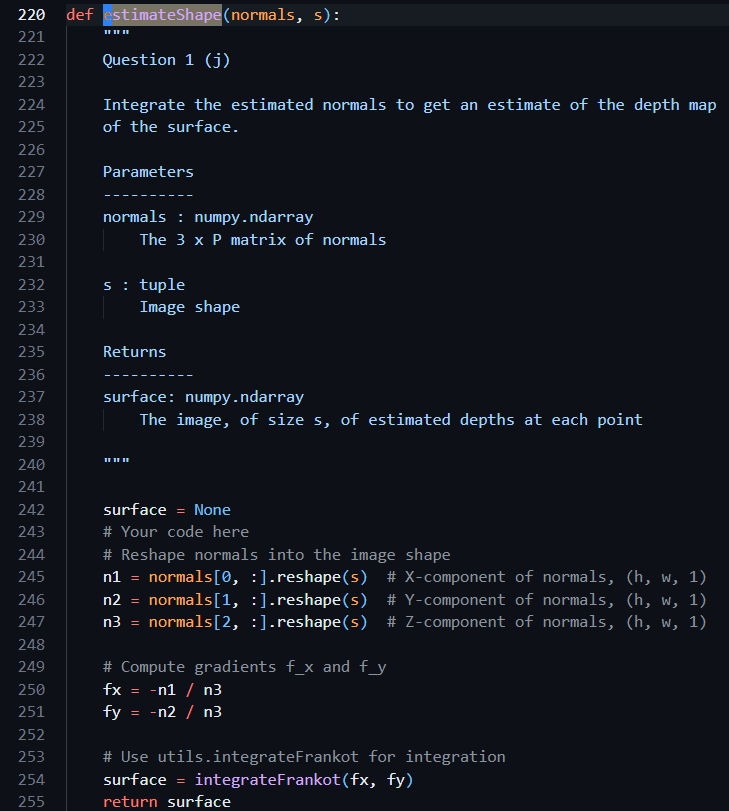
\includegraphics[width=1\columnwidth, height=1\linewidth]{./Q1_i_cns.png}
	\refstepcounter{figure}  \\% Increment the figure counter
	\textbf{Figure \thefigure:} Code Snippet % Manually add a caption/title
	\label{fig:Q1_i_cns}         % Label for referencing
	\end{minipage}	
	
	\begin{minipage}{1\linewidth}
	\centering
	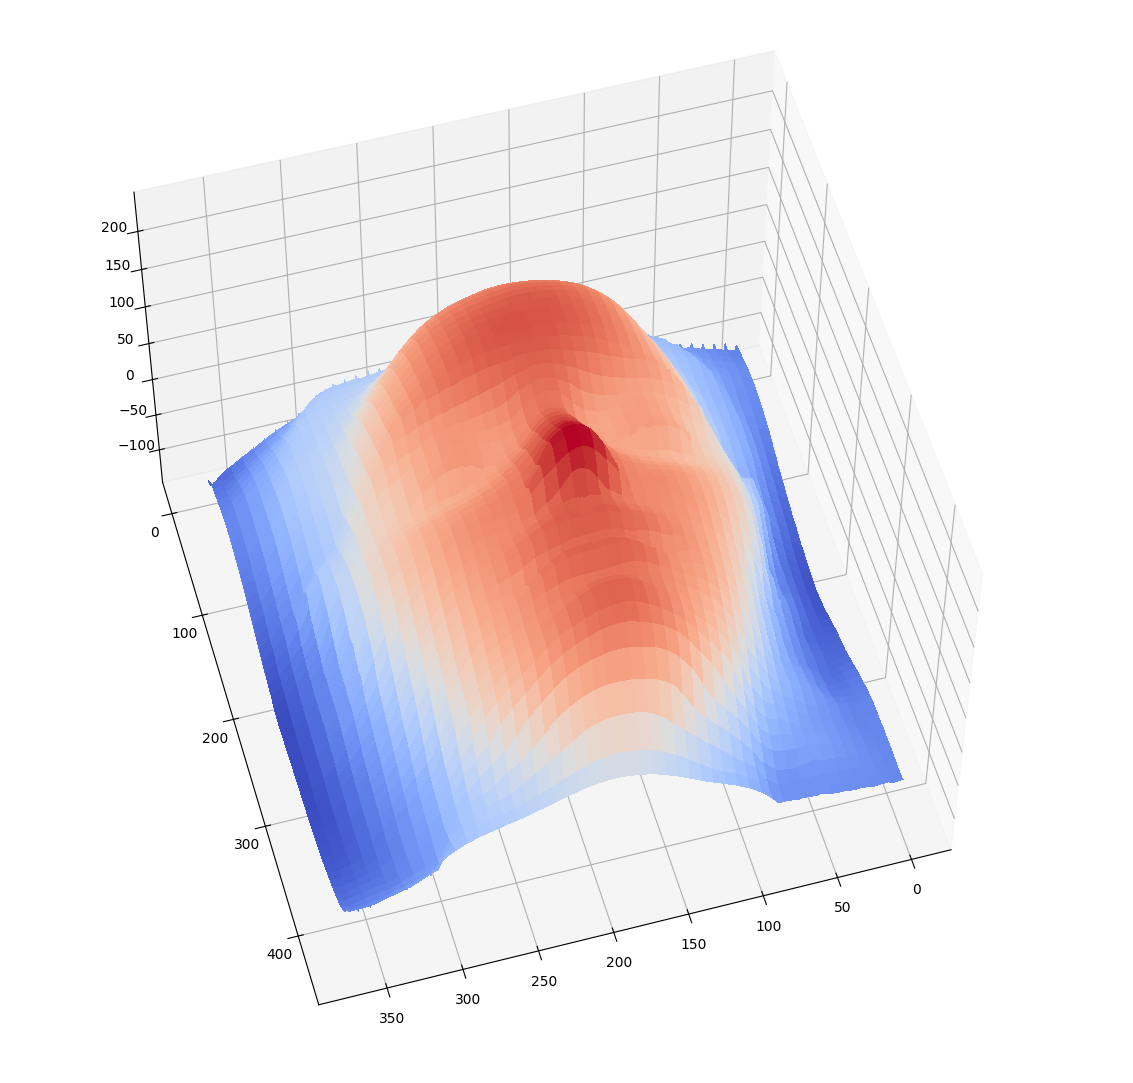
\includegraphics[width=0.8\columnwidth, height=0.6\linewidth]{./Q1_i_res1.png}
	\refstepcounter{figure}  \\% Increment the figure counter
	\textbf{Figure \thefigure:} Result of Shape Estimation in View 1  % Manually add a caption/title
	\label{fig:Q1_i_res1}         % Label for referencing
	\end{minipage}
	
	\begin{minipage}{1\linewidth}
	\centering
	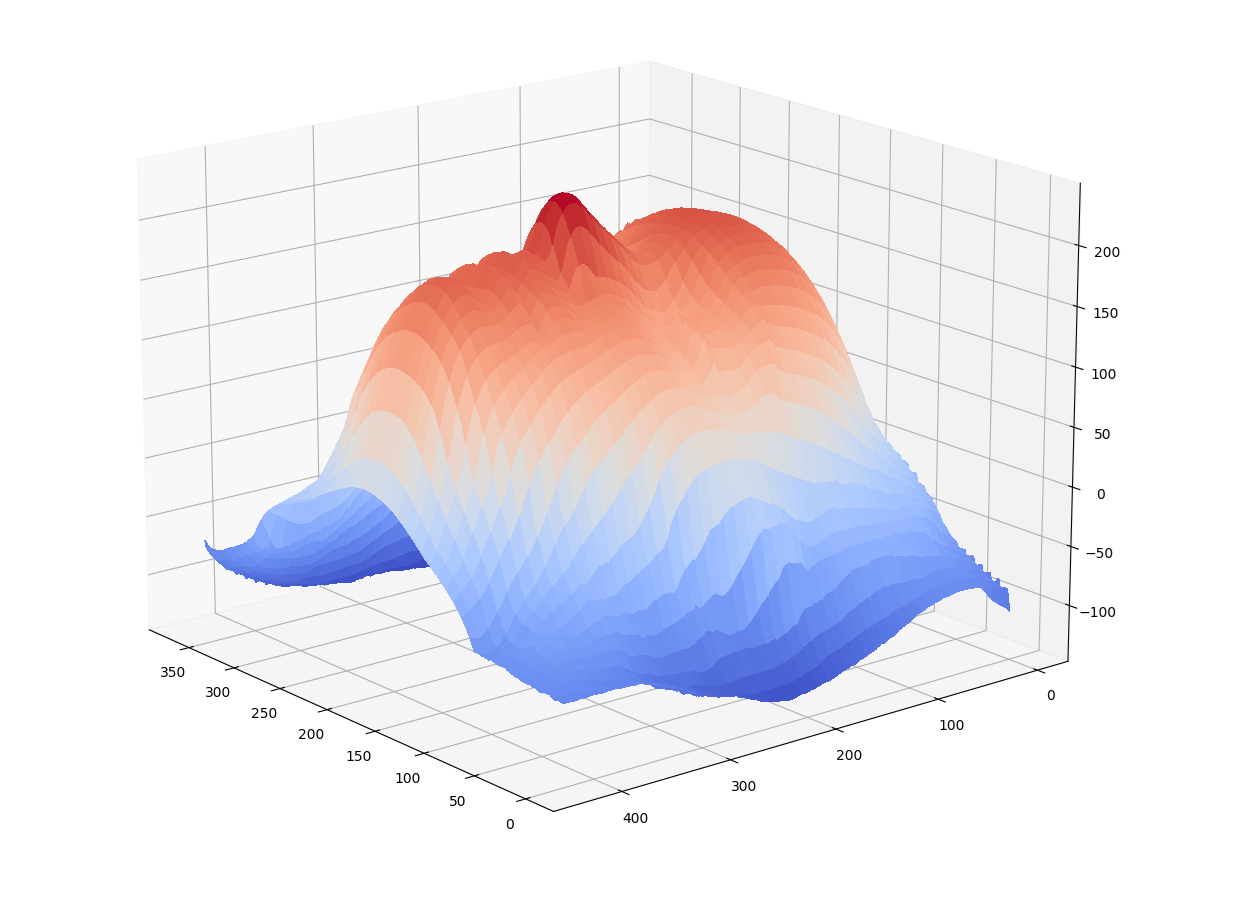
\includegraphics[width=0.8\columnwidth, height=0.6\linewidth]{./Q1_i_res2.png}
	\refstepcounter{figure}  \\% Increment the figure counter
	\textbf{Figure \thefigure:} Result of Shape Estimation in View 2  % Manually add a caption/title
	\label{fig:Q1_i_res2}         % Label for referencing
	\end{minipage}	
	
	\begin{minipage}{1\linewidth}
	\centering
	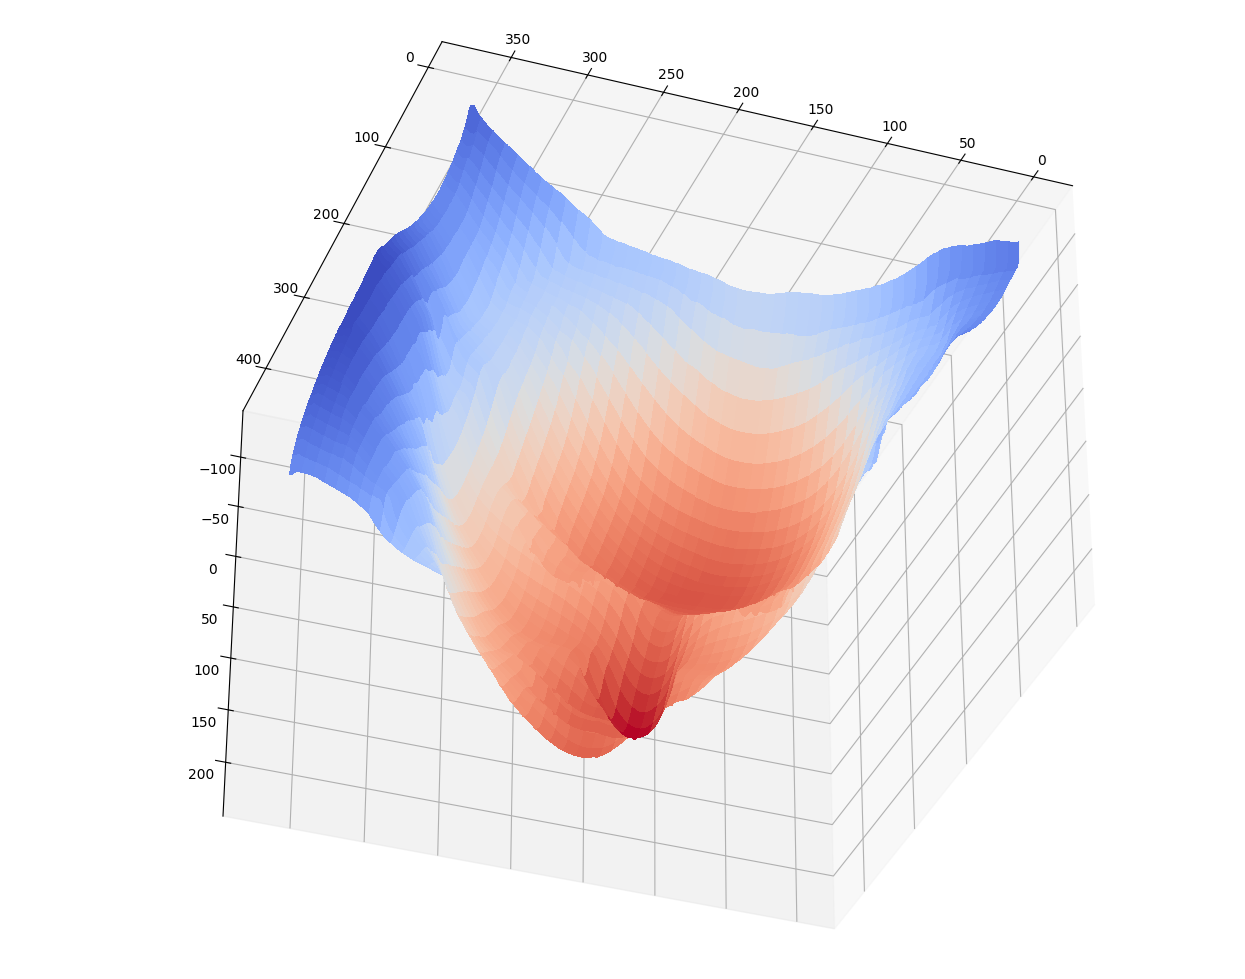
\includegraphics[width=0.8\columnwidth, height=0.6\linewidth]{./Q1_i_res3.png}
	\refstepcounter{figure}  \\% Increment the figure counter
	\textbf{Figure \thefigure:} Result of Shape Estimation in View 3  % Manually add a caption/title
	\label{fig:Q1_i_res3}         % Label for referencing
	\end{minipage}

	\newpage
	\subsection*{Q2-a at page 7}
	Ans:\\
	\hangindent=1.5em \hspace{1.5em} Since $\mathbf{I} = \mathbf{L^T}\mathbf{B}$, and we do not know $\mathbf{L^T}$ and $\mathbf{B}$, we can directly do SVD on $\mathbf{I}$. This gives:\\
	\begin{align}
		\mathbf{I} &= \mathbf{U}\mathbf{\Sigma}\mathbf{V^T}
	\end{align}
	Since $\mathbf{I}$ is a 7xP matrix, so the $\mathbf{U}$ would be a 7x7 matrix, $\Sigma$ would be a 7xP diagonal matrix, and $\mathbf{V^T}$ would be a PxP matrix, where P is the number of pixels.\\
	To approximate the rank 3 of I, we first set all singular values except the top 3 from $\mathbf{\Sigma}$ to 0, and we get the diagonal 3x3 matrix $\hat{\mathbf{\Sigma}}$. Secondly, we choose the first 3 columns of $\mathbf{U}$ to get 7x3 matrix: $\hat{\mathbf{U}}$, choose the first 3 columns of $\mathbf{V}$ to get a Px3 matrix: $\hat{\mathbf{V}}$. Thus, we can get $\hat{\mathbf{I}}$ as below:
	\begin{align}
		\hat{\mathbf{I}} &= \hat{\mathbf{U}}\hat{\mathbf{\Sigma}}\hat{\mathbf{V^T}}
	\end{align}
	Where $\hat{\mathbf{I}}$ is the reconstructed rank 3 matrix with shape 7xP. Accordingly, we can use the result of equation (22) to approximate $\hat{\mathbf{L}}^T$ and $\hat{\mathbf{B}}$:
	\begin{align}
		\hat{\mathbf{I}} &= \hat{\mathbf{U}}\hat{\mathbf{\Sigma}}^{1/2}\hat{\mathbf{\Sigma}}^{1/2}\hat{\mathbf{V^T}} \\
		                 &= \hat{\mathbf{L}}^T\hat{\mathbf{B}}
	\end{align}
	Where $\hat{\mathbf{L}}^T$ = $\hat{\mathbf{U}}\hat{\mathbf{\Sigma}}^{1/2}$ with shape 7x3, and  $\hat{\mathbf{B}}$ = $\hat{\mathbf{\Sigma}}^{1/2}\hat{\mathbf{V^T}}$ with shape 3xP. So this is how we can use SVD to approximate $\hat{\mathbf{L}}^T$ and $\hat{\mathbf{B}}$ and construct a factorization of $\hat{\mathbf{I}}$ following the required constraints of rank 3.
	
	
	\newpage
	\subsection*{Q2-b at page 7}
	Ans:\\
	\hangindent=1.5em \hspace{1.5em} Below \autoref{fig:Q2_b_a} and \autoref{fig:Q2_b_b} shows the results generated by the method mentioned in Q2-a. \autoref{fig:Q2_b_cns1} and \autoref{fig:Q2_b_cns2} show the code snippets of this question in q2.py.
	\newline
	
	\begin{minipage}{0.48\linewidth}
	\centering
	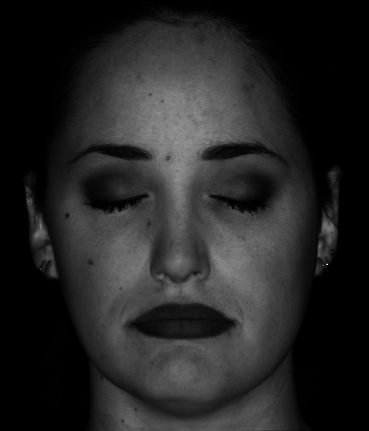
\includegraphics[width=\linewidth]{./src/2b-a.png}
	\refstepcounter{figure}  % Increment the figure counter
	\textbf{Figure \thefigure:} Estimated albedo  % Manually add a caption/title
	\label{fig:Q2_b_a}         % Label for referencing	
	\end{minipage}
\hfill
	\begin{minipage}{0.48\linewidth}
	\centering
	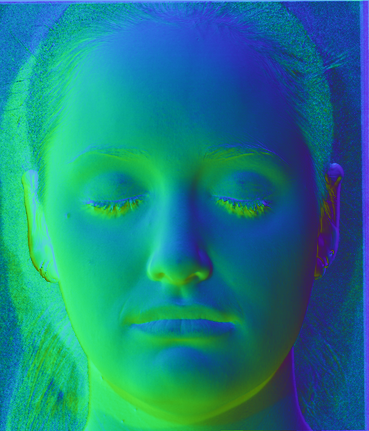
\includegraphics[width=\linewidth]{./src/2b-b.png}
	\refstepcounter{figure}  % Increment the figure counter
	\textbf{Figure \thefigure:} Estimated normals  % Manually add a caption/title
	\label{fig:Q2_b_b}         % Label for referencing
	\end{minipage}	
	\newline
	\newline
	
	\begin{minipage}{0.48\linewidth}
	\centering
	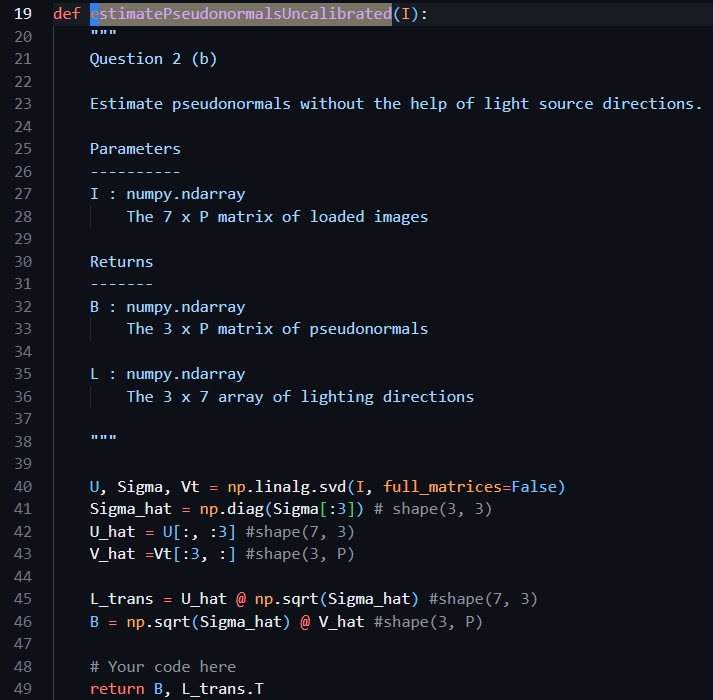
\includegraphics[width=\linewidth]{./Q2_b_cns1.png}
	\refstepcounter{figure}  % Increment the figure counter
	\textbf{Figure \thefigure:} Code Snippet 1  % Manually add a caption/title
	\label{fig:Q2_b_cns1}         % Label for referencing	
	\end{minipage}
\hfill
	\begin{minipage}{0.48\linewidth}
	\centering
	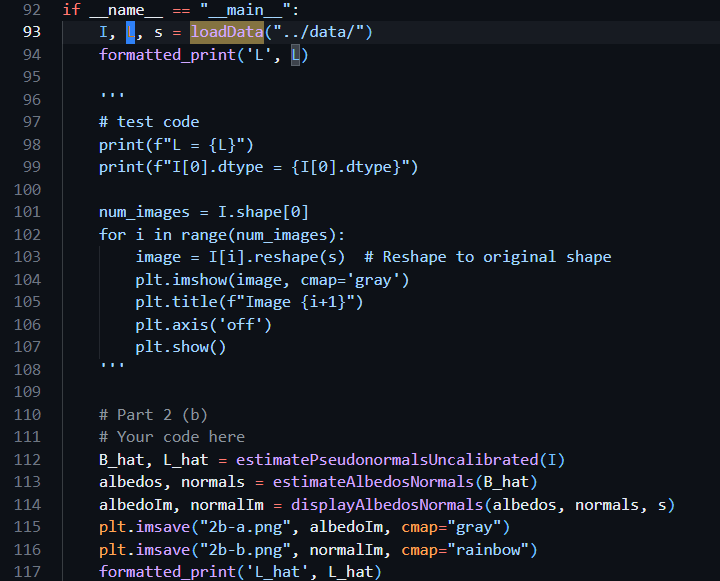
\includegraphics[width=\linewidth]{./Q2_b_cns2.png}
	\refstepcounter{figure}  % Increment the figure counter
	\textbf{Figure \thefigure:} Code Snippet 2  % Manually add a caption/title
	\label{fig:Q2_b_cns2}         % Label for referencing
	\end{minipage}

	\newpage
	\subsection*{Q2-c at page 8}
	Ans:\\
	\hangindent=1.5em \hspace{1.5em} Below \autoref{fig:Q2_c_comp_res} shows the original $\mathbf{L}$ and the reconstructed $\mathbf{\hat{L}}$ = $\mathbf{L\_hat}$. As we can see, $\mathbf{L}$ and $\mathbf{\hat{L}}$ are not similar, but quite different. There are many ways to change the procedure in (a) to change $\mathbf{\hat{L}}$ and $\mathbf{\hat{B}}$, but keeps the rendered image using them the same. For example, we can set $\hat{\mathbf{L}}^T$ = $\hat{\mathbf{U}}(\frac{1}{2}\hat{\mathbf{\Sigma}}^{1/2})$, $\hat{\mathbf{B}}$ = $(2\hat{\mathbf{\Sigma}}^{1/2})\hat{\mathbf{V^T}}$, and $\hat{\mathbf{L}}^T\hat{\mathbf{B}}$, the rendered image, is still the same.
	\newline

	\begin{minipage}{1\linewidth}
	\centering
	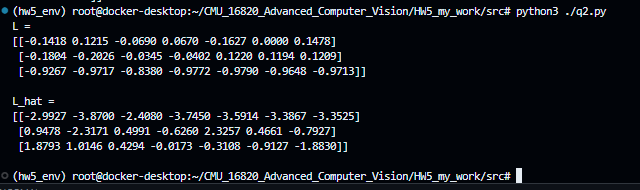
\includegraphics[width=0.8\columnwidth, height=0.3\linewidth]{./Q2_c_comp_res.png}
	\refstepcounter{figure}  \\% Increment the figure counter
	\textbf{Figure \thefigure:} Comparison of $\mathbf{L}$ and $\mathbf{\hat{L}}$  % Manually add a caption/title
	\label{fig:Q2_c_comp_res}         % Label for referencing
	\end{minipage}
	
	\newpage
	\subsection*{Q2-d at page 8}
	Ans:\\
	\hangindent=1.5em \hspace{1.5em} \autoref{fig:Q2_d_res1} and \autoref{fig:Q2_d_res2} show different views of the reconstructed 3D depth map shape using Franot-Chellappa algorithm. It does not look like a face.
	\newline
	
	\begin{minipage}{0.48\linewidth}
	\centering
	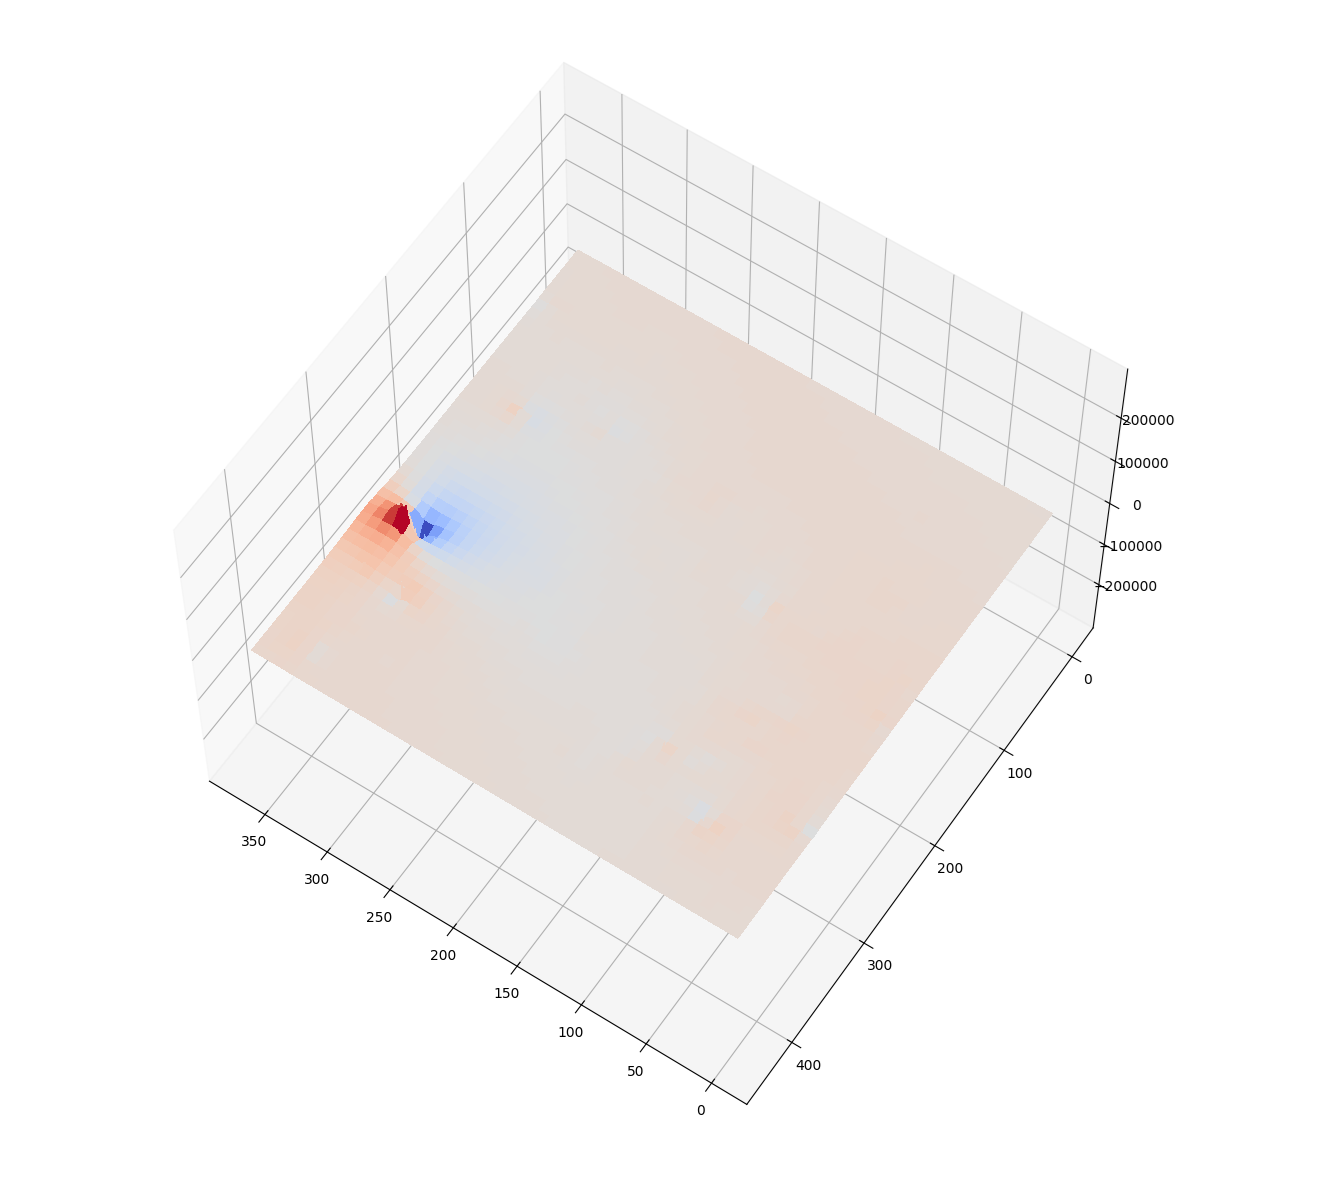
\includegraphics[width=\linewidth]{./Q2_d_res1.png}
	\refstepcounter{figure}  % Increment the figure counter
	\textbf{Figure \thefigure:} Reconstructed 3D Depth Map Shape View1  % Manually add a caption/title
	\label{fig:Q2_d_res1}         % Label for referencing	
	\end{minipage}
\hfill
	\begin{minipage}{0.48\linewidth}
	\centering
	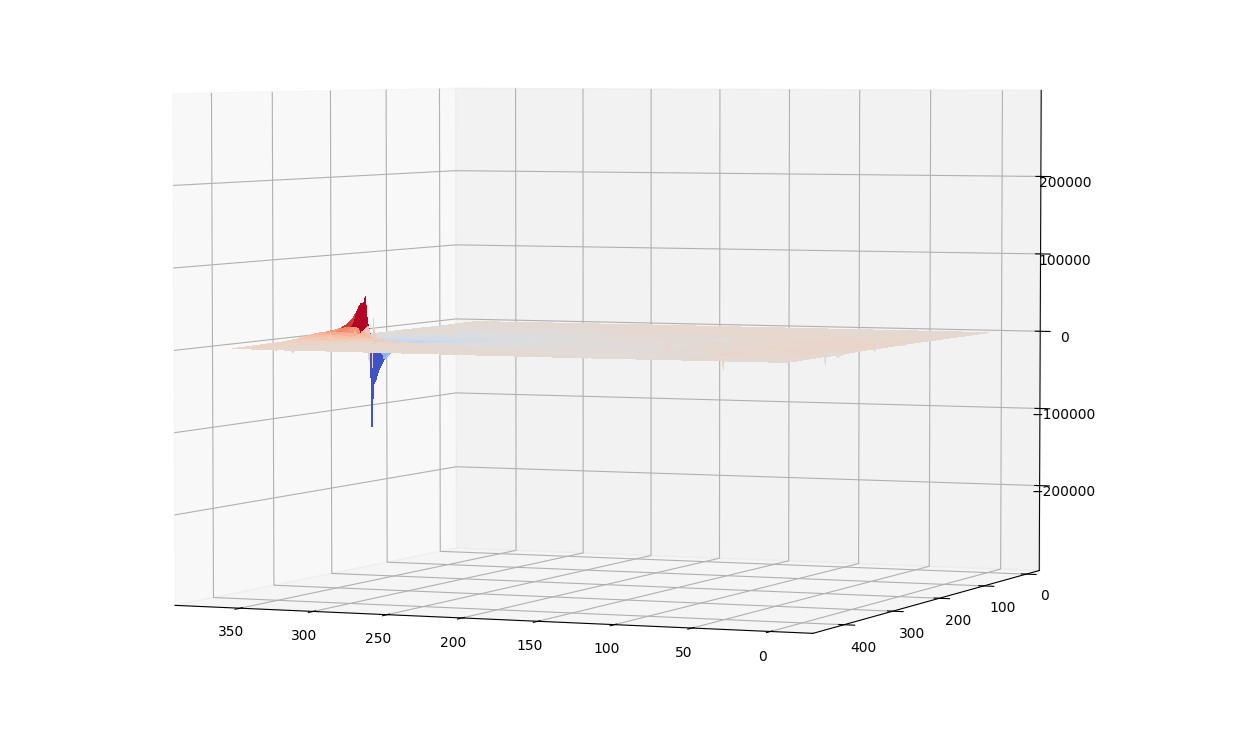
\includegraphics[width=\linewidth]{./Q2_d_res2.png}
	\refstepcounter{figure}  % Increment the figure counter
	\textbf{Figure \thefigure:} Reconstructed 3D Depth Map Shape View2  % Manually add a caption/title
	\label{fig:Q2_d_res2}         % Label for referencing
	\end{minipage}
	
	\newpage
	\subsection*{Q2-e at page 8}
	Ans:\\
	\hangindent=1.5em \hspace{1.5em}The following \autoref{fig:Q2_e_res1} - \autoref{fig:Q2_e_res3} show the results of estimated shape in three different viewpoints using pseudonormals and enforceIntegrability() in utils.py. The surface does look like the one output by calibrated photometric stereo in Q1-i question above, but it seems to be a little more flattened, as one can see the height range of the results here are only in the range of [-50, 100], while the results in Q1-i are in the range of [-100, 200].


	\begin{minipage}{1\linewidth}
	\centering
	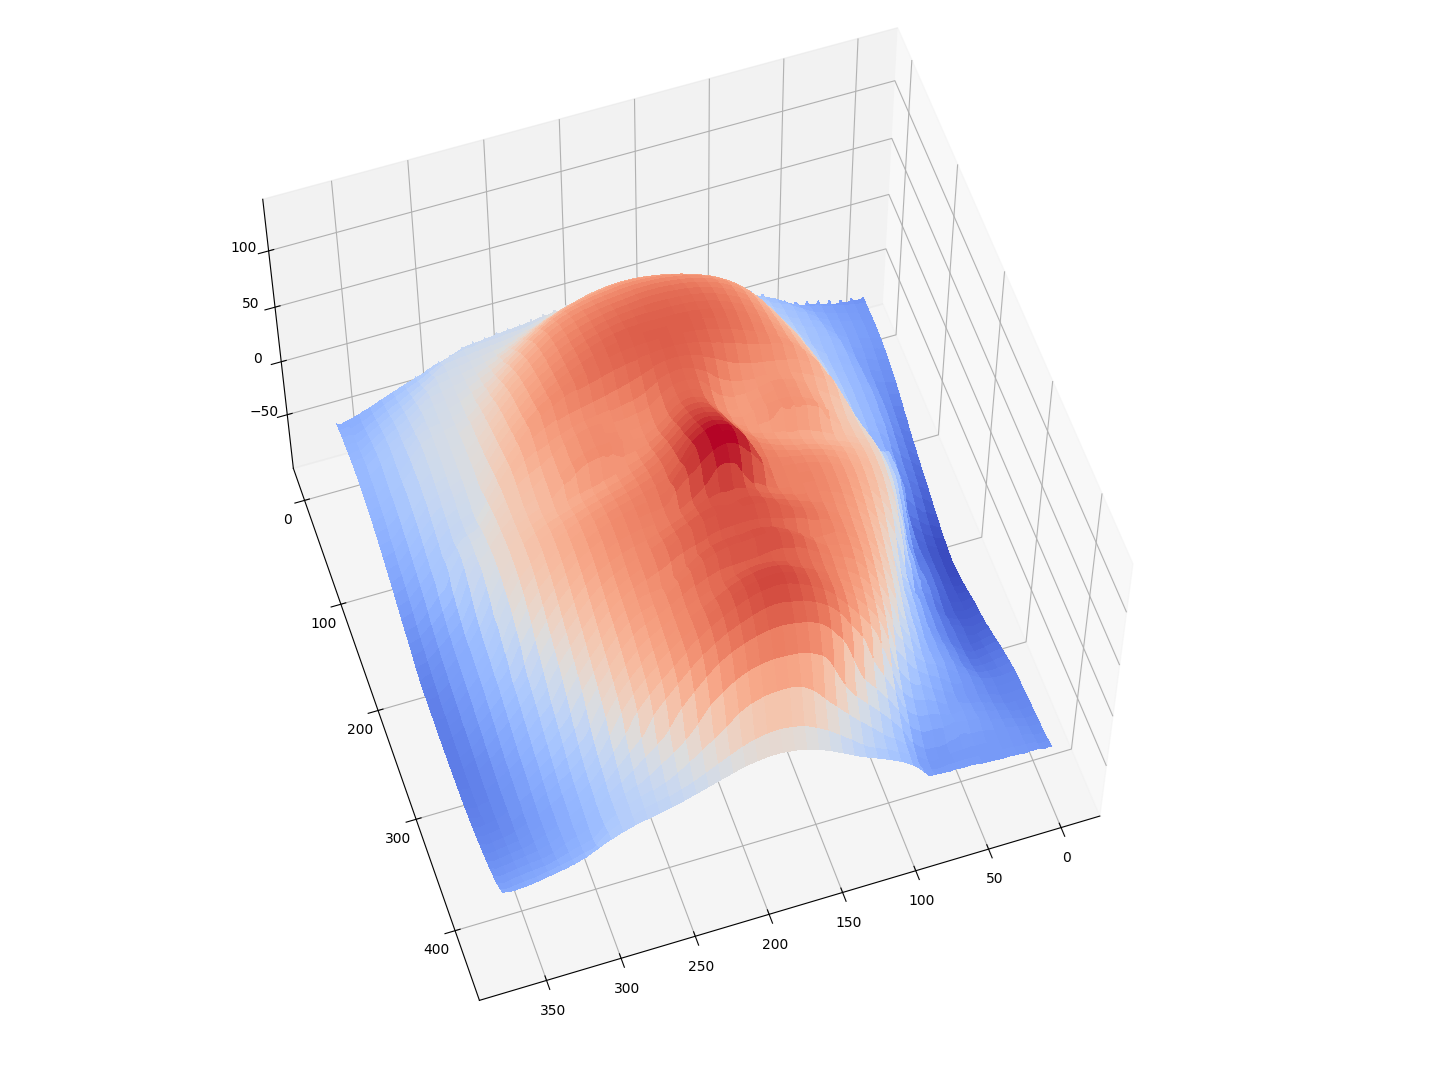
\includegraphics[width=0.8\columnwidth, height=0.6\linewidth]{./Q2_e_res1.png}
	\refstepcounter{figure}  \\% Increment the figure counter
	\textbf{Figure \thefigure:} Result of Shape Estimation in View 1  % Manually add a caption/title
	\label{fig:Q2_e_res1}         % Label for referencing
	\end{minipage}

	\begin{minipage}{1\linewidth}
	\centering
	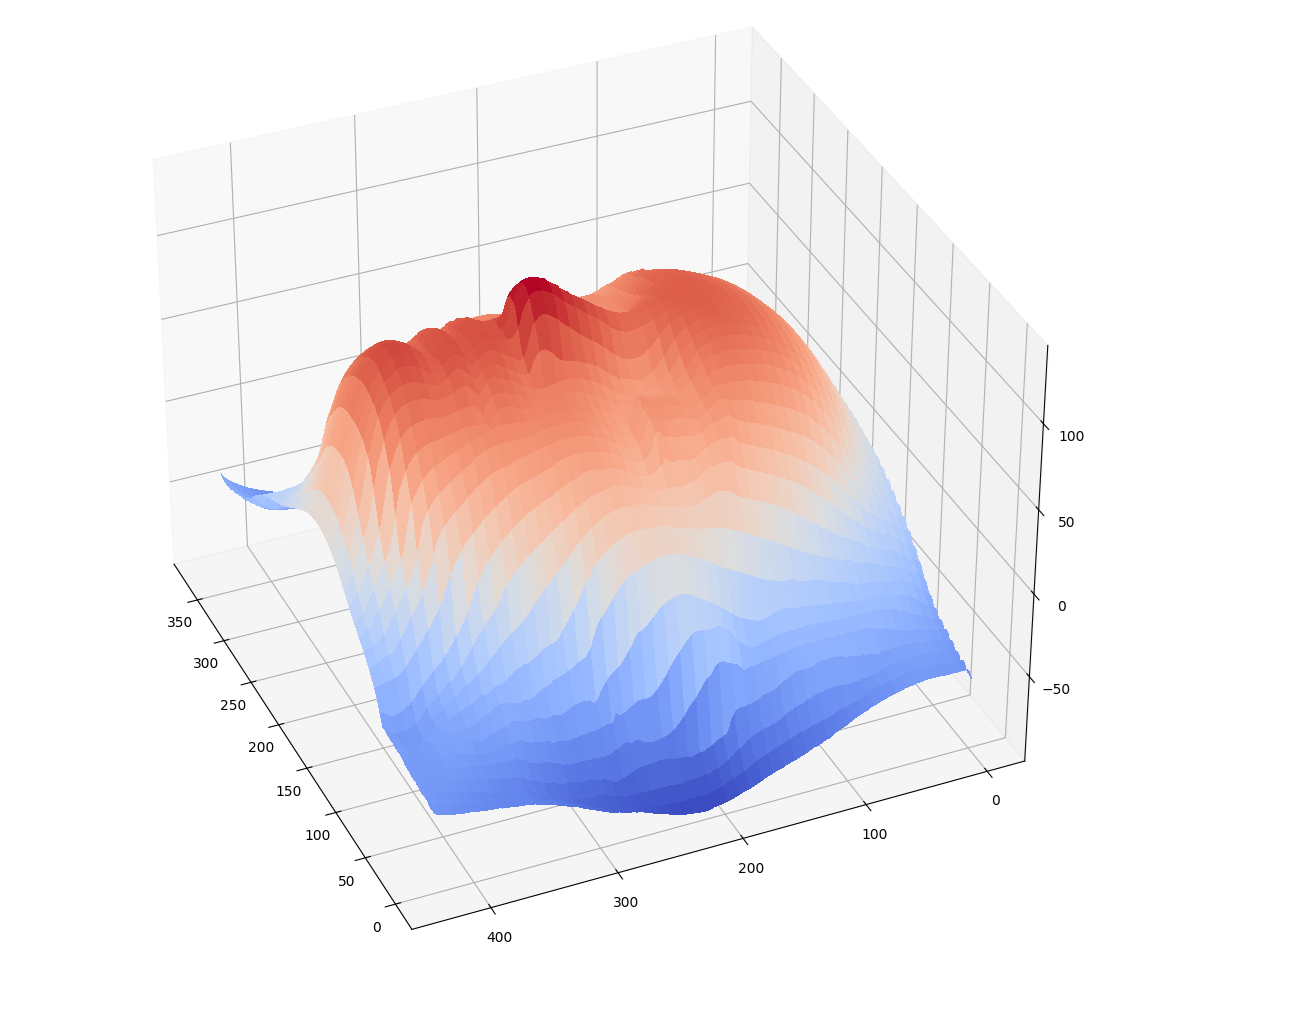
\includegraphics[width=0.8\columnwidth, height=0.6\linewidth]{./Q2_e_res2.png}
	\refstepcounter{figure}  \\% Increment the figure counter
	\textbf{Figure \thefigure:} Result of Shape Estimation in View 2  % Manually add a caption/title
	\label{fig:Q2_e_res2}         % Label for referencing
	\end{minipage}	

	\begin{minipage}{1\linewidth}
	\centering
	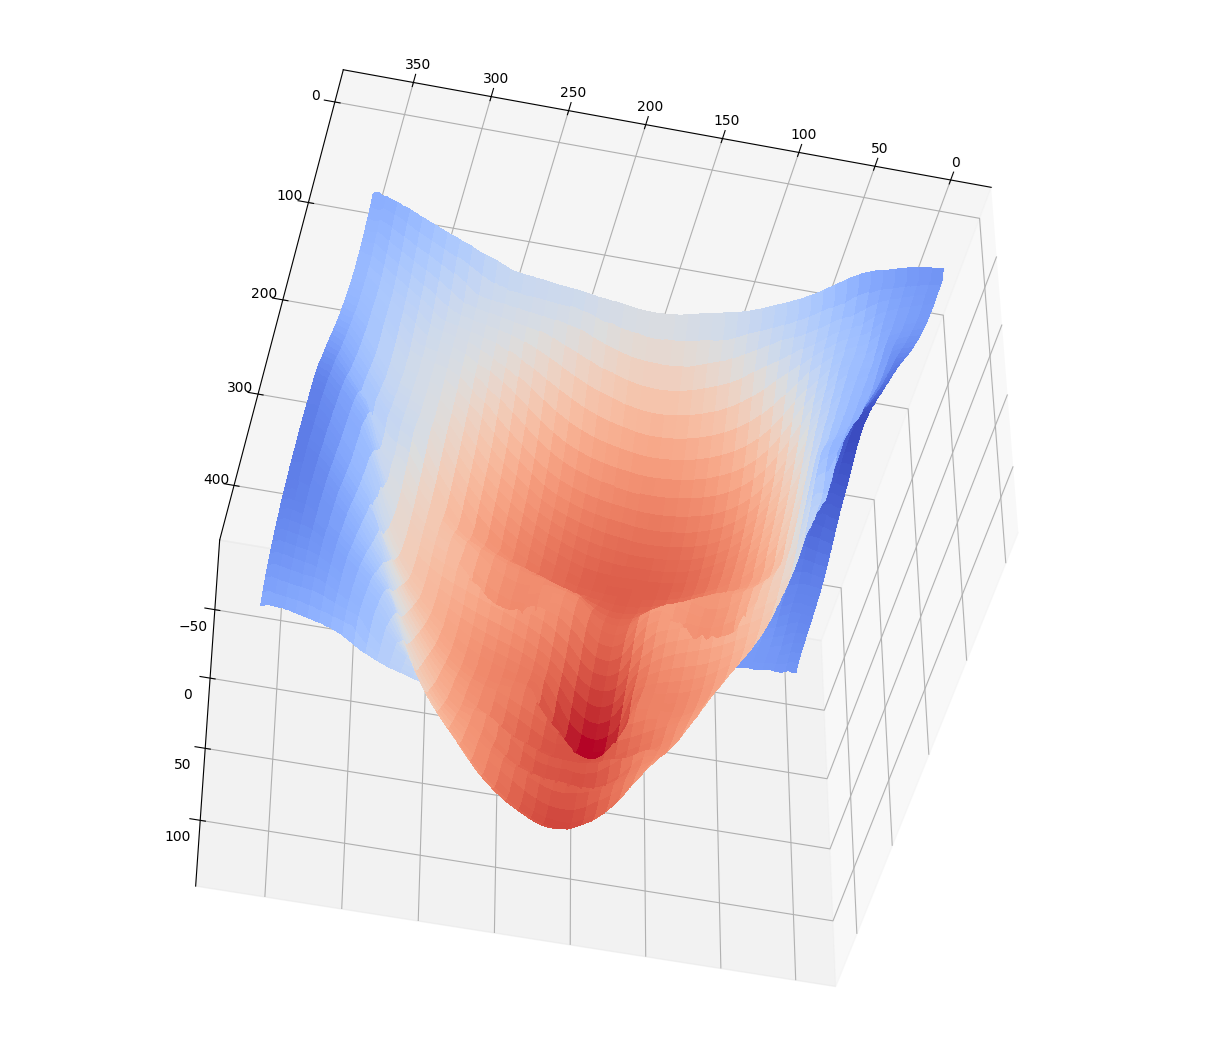
\includegraphics[width=0.8\columnwidth, height=0.6\linewidth]{./Q2_e_res3.png}
	\refstepcounter{figure}  \\% Increment the figure counter
	\textbf{Figure \thefigure:} Result of Shape Estimation in View 3  % Manually add a caption/title
	\label{fig:Q2_e_res3}         % Label for referencing
	\end{minipage}
	
	\newpage
	\subsection*{Q2-f at page 9}
	Ans:\\
	\hangindent=1.5em \hspace{1.5em}Let's discuss how the value of $\mu$ $\nu$ $\lambda$ affect the reconstructed surface: \\
	When $\mu$ = [-0.1, -1, -10], and $\nu$ = 1, $\lambda$ = 1: \\
\begin{figure}[H]
	\centering
	% First image
	\begin{subfigure}{0.33\textwidth}
		\centering
		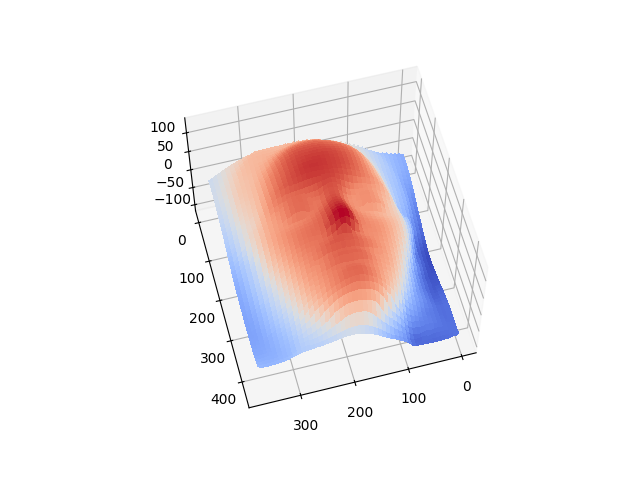
\includegraphics[width=\textwidth]{./src/2f_mu_change/faceCalibrated_mu_-0.1_v_1_lambda_1.png}
		\caption{$\mu$=-0.1, $\nu$=1, $\lambda$=1}
	\end{subfigure}
	\hfill
	% Second image
	\begin{subfigure}{0.32\textwidth}
		\centering
		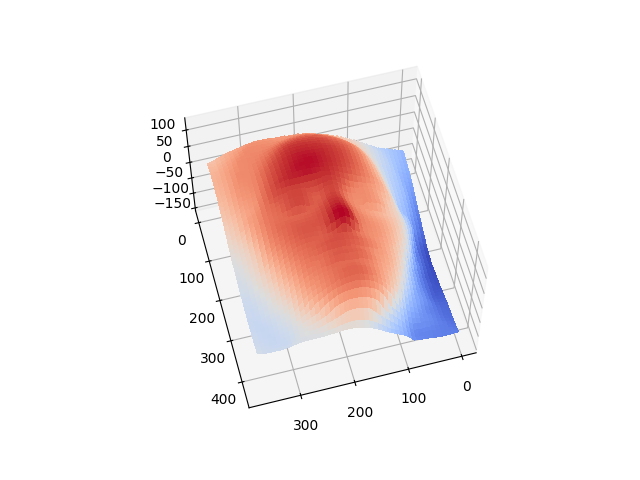
\includegraphics[width=\textwidth]{./src/2f_mu_change/faceCalibrated_mu_-1_v_1_lambda_1.png}
		\caption{$\mu$=-1, $\nu$=1, $\lambda$=1}
	\end{subfigure}
	\hfill
	% Third image
	\begin{subfigure}{0.32\textwidth}
		\centering
		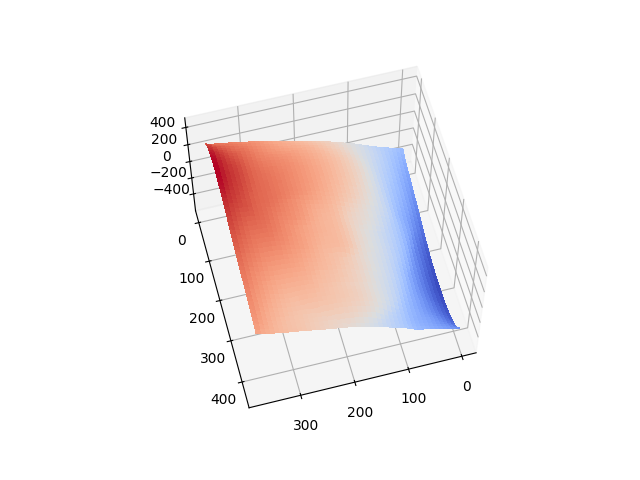
\includegraphics[width=\textwidth]{./src/2f_mu_change/faceCalibrated_mu_-10_v_1_lambda_1.png}
		\caption{$\mu$=-10, $\nu$=1, $\lambda$=1}
	\end{subfigure}
	
	\caption{Impact of Negative $\mu$ Values on Surface}
	\label{fig:u_n_vl}
\end{figure}

	\hangindent=1.5em \hspace{1.5em}When $\mu$ = [0.1, 1, 10], and $\nu$ = 1, $\lambda$ = 1: \\
\begin{figure}[H]
	\centering
	% First image
	\begin{subfigure}{0.33\textwidth}
		\centering
		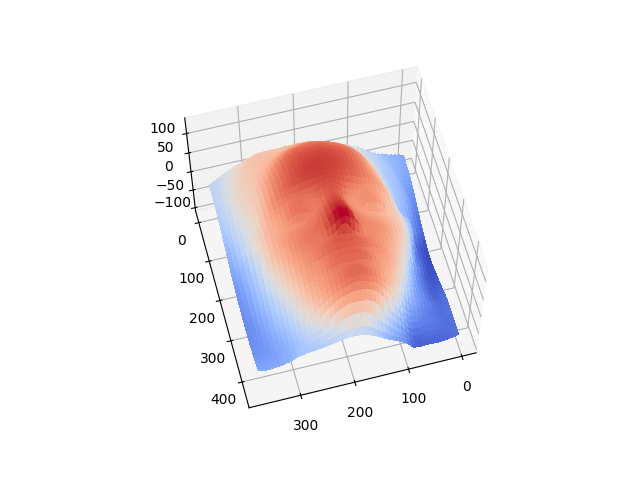
\includegraphics[width=\textwidth]{./src/2f_mu_change/faceCalibrated_mu_0.1_v_1_lambda_1.png}
		\caption{$\mu$=0.1, $\nu$=1, $\lambda$=1}
	\end{subfigure}
	\hfill
	% Second image
	\begin{subfigure}{0.32\textwidth}
		\centering
		\includegraphics[width=\textwidth]{./src/2f_mu_change/faceCalibrated_mu_1_v_1_lambda_1.png}
		\caption{$\mu$=1, $\nu$=1, $\lambda$=1}
	\end{subfigure}
	\hfill
	% Third image
	\begin{subfigure}{0.32\textwidth}
		\centering
		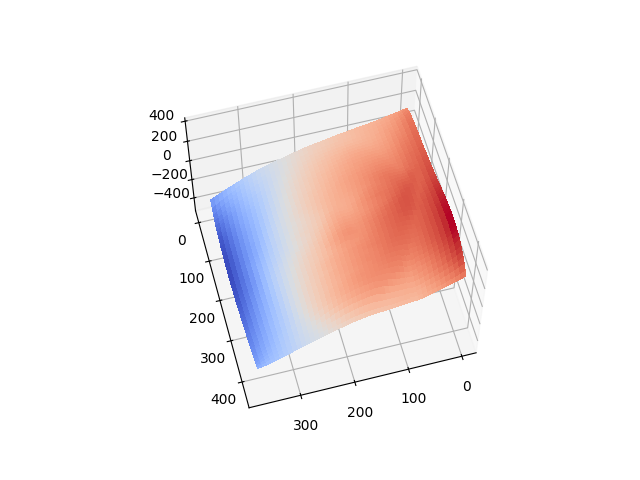
\includegraphics[width=\textwidth]{./src/2f_mu_change/faceCalibrated_mu_10_v_1_lambda_1.png}
		\caption{$\mu$=10, $\nu$=1, $\lambda$=1}
	\end{subfigure}
	
	\caption{Impact of Positive $\mu$ Values on Surface}
	\label{fig:u_p_vl}
\end{figure}

	\hangindent=1.5em \hspace{1.5em}When $\nu$ = [-0.1, -1, -10], and $\mu$ = 1, $\lambda$ = 1: \\
\begin{figure}[H]
	\centering
	% First image
	\begin{subfigure}{0.33\textwidth}
		\centering
		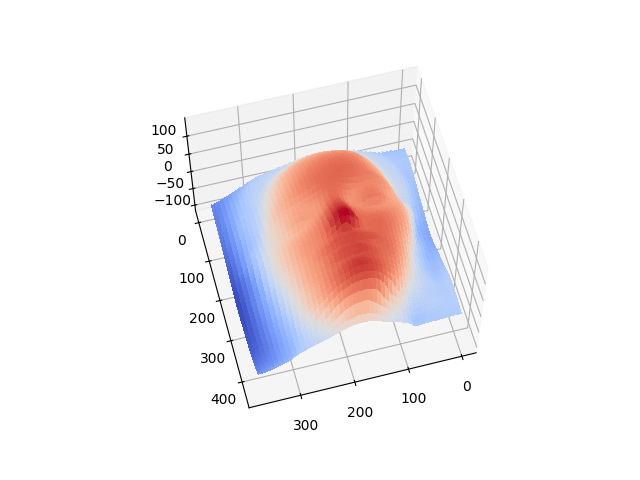
\includegraphics[width=\textwidth]{./src/2f_v_change/faceCalibrated_mu_1_v_-0.1_lambda_1.png}
		\caption{$\mu$=1, $\nu$=-0.1, $\lambda$=1}
	\end{subfigure}
	\hfill
	% Second image
	\begin{subfigure}{0.32\textwidth}
		\centering
		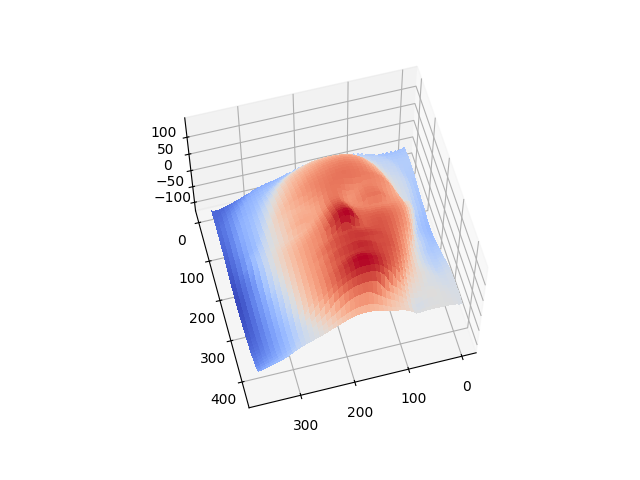
\includegraphics[width=\textwidth]{./src/2f_v_change/faceCalibrated_mu_1_v_-1_lambda_1.png}
		\caption{$\mu$=1, $\nu$=-1, $\lambda$=1}
	\end{subfigure}
	\hfill
	% Third image
	\begin{subfigure}{0.32\textwidth}
		\centering
		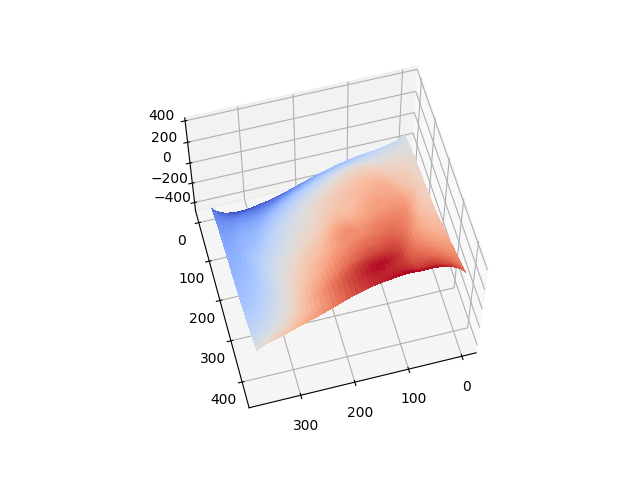
\includegraphics[width=\textwidth]{./src/2f_v_change/faceCalibrated_mu_1_v_-10_lambda_1.png}
		\caption{$\mu$=1, $\nu$=-10, $\lambda$=1}
	\end{subfigure}
	
	\caption{Impact of Negative $\nu$ Values on Surface}
	\label{fig:v_n_ul}
\end{figure}
	
	\hangindent=1.5em \hspace{1.5em}When $\nu$ = [0.1, 1, 10], and $\mu$ = 1, $\lambda$ = 1: \\
\begin{figure}[H]
	\centering
	% First image
	\begin{subfigure}{0.33\textwidth}
		\centering
		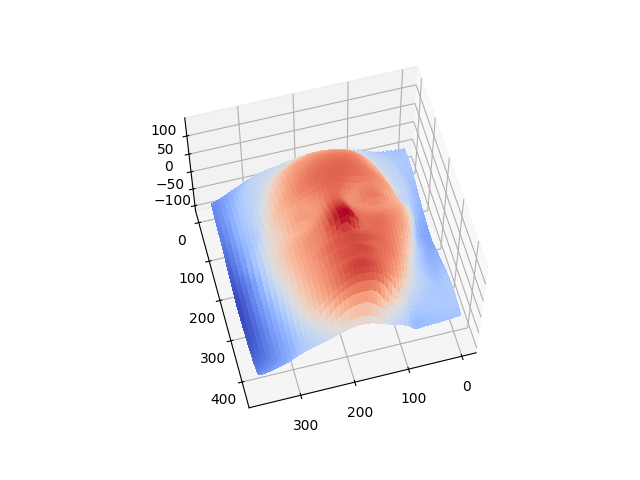
\includegraphics[width=\textwidth]{./src/2f_v_change/faceCalibrated_mu_1_v_0.1_lambda_1.png}
		\caption{$\mu$=1, $\nu$=0.1, $\lambda$=1}
	\end{subfigure}
	\hfill
	% Second image
	\begin{subfigure}{0.32\textwidth}
		\centering
		\includegraphics[width=\textwidth]{./src/2f_v_change/faceCalibrated_mu_1_v_1_lambda_1.png}
		\caption{$\mu$=1, $\nu$=1, $\lambda$=1}
	\end{subfigure}
	\hfill
	% Third image
	\begin{subfigure}{0.32\textwidth}
		\centering
		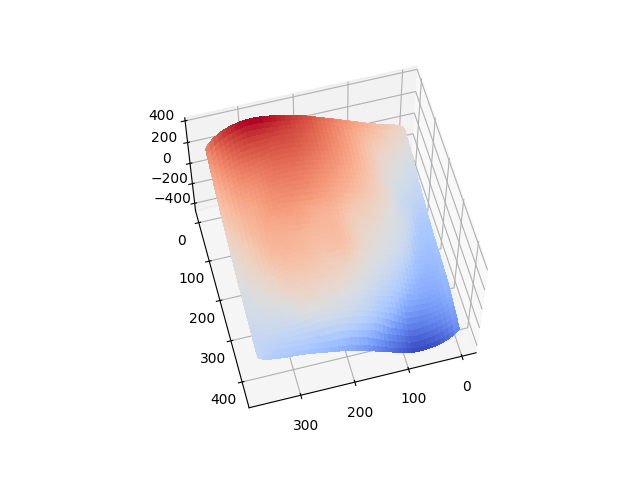
\includegraphics[width=\textwidth]{./src/2f_v_change/faceCalibrated_mu_1_v_10_lambda_1.png}
		\caption{$\mu$=1, $\nu$=10, $\lambda$=1}
	\end{subfigure}
	
	\caption{Impact of Positive $\nu$ Values on Surface}
	\label{fig:v_p_ul}
\end{figure}	
	\hangindent=1.5em \hspace{1.5em}When $\lambda$ = [-0.1, -1, -10], and $\mu$ = 1, $\nu$ = 1: \\
\begin{figure}[H]
	\centering
	% First image
	\begin{subfigure}{0.33\textwidth}
		\centering
		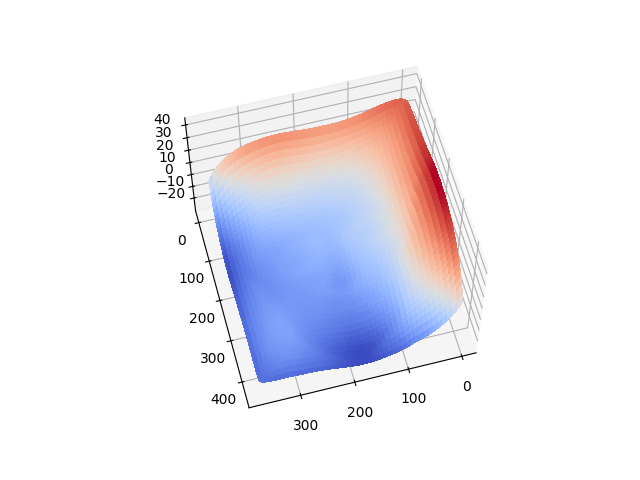
\includegraphics[width=\textwidth]{./src/2f_lambda_change/faceCalibrated_mu_1_v_1_lambda_-0.1.png}
		\caption{$\mu$=1, $\nu$=1, $\lambda$=-0.1}
	\end{subfigure}
	\hfill
	% Second image
	\begin{subfigure}{0.32\textwidth}
		\centering
		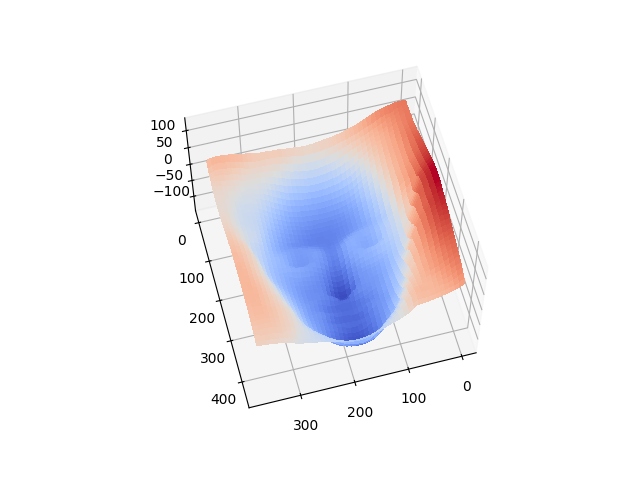
\includegraphics[width=\textwidth]{./src/2f_lambda_change/faceCalibrated_mu_1_v_1_lambda_-1.png}
		\caption{$\mu$=1, $\nu$=1, $\lambda$=-1}
	\end{subfigure}
	\hfill
	% Third image
	\begin{subfigure}{0.32\textwidth}
		\centering
		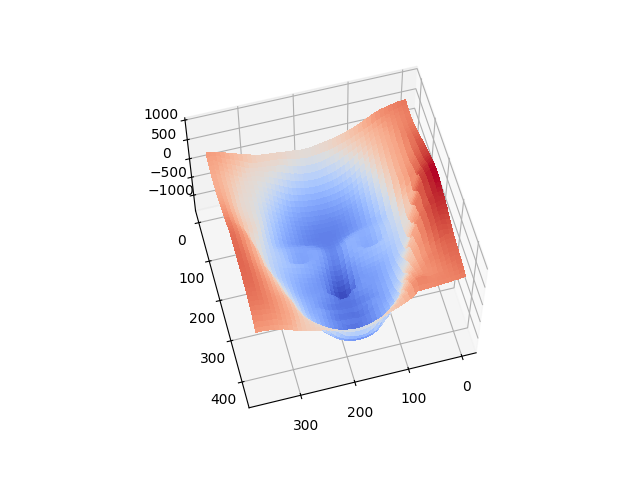
\includegraphics[width=\textwidth]{./src/2f_lambda_change/faceCalibrated_mu_1_v_1_lambda_-10.png}
		\caption{$\mu$=1, $\nu$=1, $\lambda$=-10}
	\end{subfigure}
	
	\caption{Impact of Negative $\lambda$ Values on Surface}
	\label{fig:l_n_uv}
\end{figure}
	
	\hangindent=1.5em \hspace{1.5em}When $\lambda$ = [0.1, 1, 10], and $\mu$ = 1, $\nu$ = 1: \\
\begin{figure}[H]
	\centering
	% First image
	\begin{subfigure}{0.33\textwidth}
		\centering
		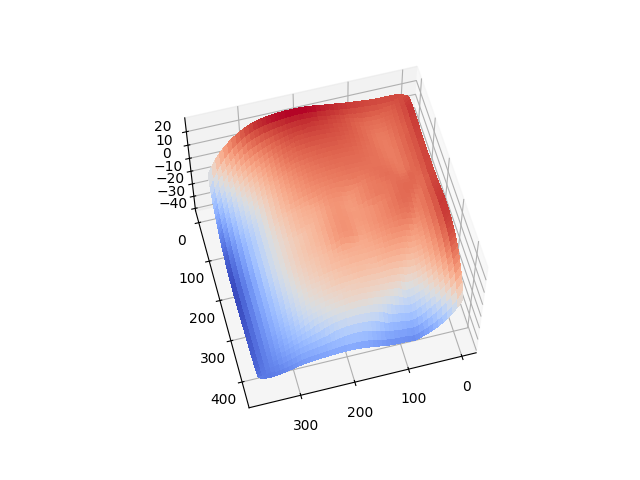
\includegraphics[width=\textwidth]{./src/2f_lambda_change/faceCalibrated_mu_1_v_1_lambda_0.1.png}
		\caption{$\mu$=1, $\nu$=1, $\lambda$=0.1}
	\end{subfigure}
	\hfill
	% Second image
	\begin{subfigure}{0.32\textwidth}
		\centering
		\includegraphics[width=\textwidth]{./src/2f_lambda_change/faceCalibrated_mu_1_v_1_lambda_1.png}
		\caption{$\mu$=1, $\nu$=1, $\lambda$=1}
	\end{subfigure}
	\hfill
	% Third image
	\begin{subfigure}{0.32\textwidth}
		\centering
		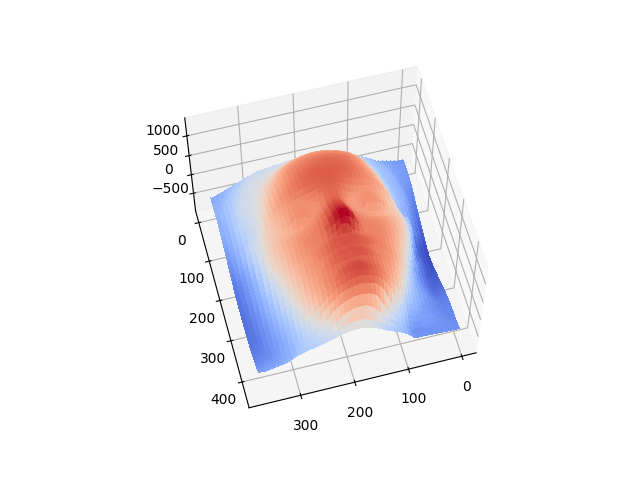
\includegraphics[width=\textwidth]{./src/2f_lambda_change/faceCalibrated_mu_1_v_1_lambda_10.png}
		\caption{$\mu$=1, $\nu$=1, $\lambda$=10}
	\end{subfigure}
	
	\caption{Impact of Positive $\lambda$ Values on Surface}
	\label{fig:l_p_uv}
\end{figure}
	\hangindent=1.5em \hspace{1.5em}As we can see above, when $\mu$ changes from small values to large values, the surface gets more flattened, while the positive and negative values affect the surface to be more flattened toward opposite directions. The $\nu$ changes in similar way, as it changes from small values to large values, the surface gets more flattened, while the positive and negative values affect the surface to be more flattened in opposite directions. The $\lambda$ changes in another particular way: as its value change from small to large, the curve of the surface becomes sharper, while the positive and negative values affect the surface to be sharper in opposite directions.\\
	\hangindent=1.5em \hspace{1.5em}The reason why bas-relief ambiguity is named so is that the GBR transform preserves the dot product of surface normal and light direction while producing different surface shape by tilting and scaling curved depth (the x and y components of B are not changed, only z component becomes the combination of x, y and z components after GBR transform), which can be seen from above \autoref{fig:u_n_vl} to \autoref{fig:l_p_uv}. That is to say, $\mathbf{I}$, which is $\mathbf{L}^T\mathbf{B}$, would be equal to $\mathbf{I'}$ = $\mathbf{L}^T\mathbf{B'}$, where $\mathbf{B'} = \mathbf{G^{-T}}\mathbf{B}$, because the appearance $\mathbf{I}$ only depends on the $\cos\theta$ between $\mathbf{L}$ and $\mathbf{B}$. As a result, we cannot reconstruct a unique shape based only on appearance $\mathbf{I}$.
	
	\newpage
	\subsection*{Q2-g at page 9}
	Ans:\\
	\hangindent=1.5em \hspace{1.5em}As we can see the trend in Q2-f, the larger absolute value of $\mu$ or $\nu$, not both, the more flattened the reconstructed shape is. Besides, the smaller absolute value of $\lambda$, the more flattened the reconstructed shape is. Thus, we can use the setting of $\mu$ = 10, $\nu$ = 1, and $\lambda$=0.001 to generate the flattened shape as below \autoref{fig:Q2_g_res}. 

	\begin{minipage}{1\linewidth}
	\centering
	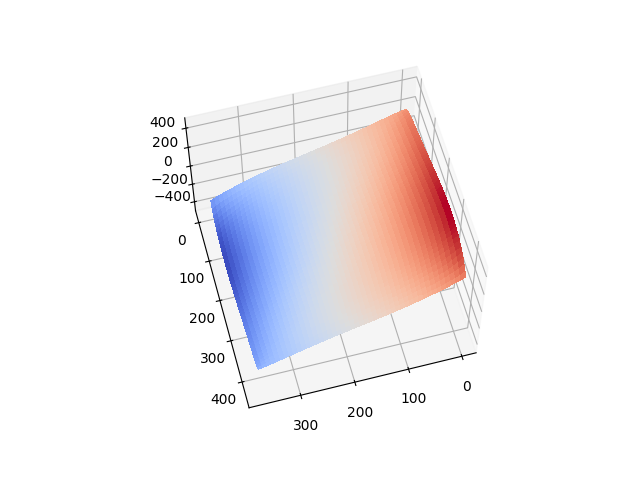
\includegraphics[width=0.8\columnwidth, height=0.6\linewidth]{./src/2g_flattest_result/faceCalibrated_mu_10_v_1_lambda_0.001.png}
	\refstepcounter{figure}  \\% Increment the figure counter
	\textbf{Figure \thefigure:} Result of Flattened Shape % Manually add a caption/title
	\label{fig:Q2_g_res}         % Label for referencing
	\end{minipage}
	\newline
	
	\hangindent=0.4em \hspace{0.3em}Another interesting fact is that when we set both $\mu$ and $\nu$ to be large, the reconstructed shape would not be flattened:
\begin{figure}[H]	
	\begin{subfigure}{0.33\textwidth}
	\centering
	\includegraphics[width=\textwidth]{./src/2g_all_change/faceCalibrated_mu_1_v_1_lambda_1.png}
	\caption{$\mu$=1, $\nu$=1}
	\end{subfigure}
	\hfill
% Second image
	\begin{subfigure}{0.32\textwidth}
	\centering
	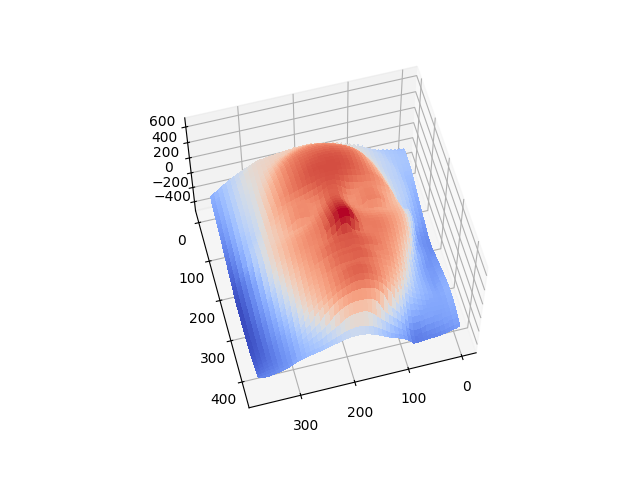
\includegraphics[width=\textwidth]{./src/2g_all_change/faceCalibrated_mu_5_v_5_lambda_5.png}
	\caption{$\mu$=5, $\nu$=5}
	\end{subfigure}
	\hfill
% Third image
	\begin{subfigure}{0.32\textwidth}
	\centering
	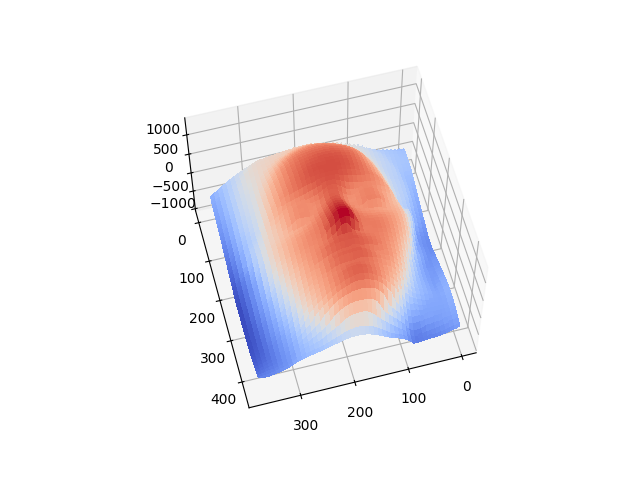
\includegraphics[width=\textwidth]{./src/2g_all_change/faceCalibrated_mu_10_v_10_lambda_10.png}
	\caption{$\mu$=10, $\nu$=10}
	\end{subfigure}	
\end{figure}

	\newpage
	\subsection*{Q2-h at page 9}
	Ans:\\
	\hangindent=1.5em \hspace{1.5em}Acquiring more pictures does not help resolve the ambiguity, because with only known appearance $\mathbf{I}$, we can only calculate the reconstructed $\mathbf{B}$ up to a matrix of the form in Eq. 2 above, the GBR transform, generating the same appearance as original $\mathbf{B}$ does. To resolve the ambiguity, we may need the light direction $\mathbf{L}$, the depth information, or other features like the geometry of the object.



	\newpage
	\subsection*{Collaborations}
	Ans:\\
	\hangindent=0.4em \hspace{0.3em} Though I do not have collaborators, I found the following websites helpful on understanding the concepts in this homework.
	\begin{enumerate}
		\item \url{https://www.ri.cmu.edu/pub_files/pub3/baker_simon_2003_3/baker_simon_2003_3.pdf.}
		\item \url{https://www2.eecs.berkeley.edu/Research/Projects/CS/vision/classes/cs294-appearance_models/sp2001/cache/belhumeur99.pdf}
		\item \url{https://matplotlib.org/stable/api/_as_gen/matplotlib.pyplot.imsave.html}	
		\item \url{https://https://en.wikipedia.org/wiki/Singular_value_decomposition}	
		\item \url{http://graphics.cs.cmu.edu/courses/15-463/2019_fall/lectures/lecture16.pdf}
	\end{enumerate}

\end{document}